\documentclass[11pt,a4paper,oneside]{report}

\usepackage[utf8]{inputenc}
\usepackage[T1]{fontenc}
\usepackage[italian]{babel}
\usepackage{lmodern}
\usepackage{microtype}
\usepackage{graphicx}
\usepackage{float}
\usepackage{caption}
\captionsetup{font={small,sf}, labelfont=bf}
\usepackage[top=2.5cm, bottom=2.5cm, left=2.5cm, right=2.5cm]{geometry}

\usepackage{amsmath,amssymb,amsthm,mathtools,bm}
\usepackage{booktabs}
\usepackage{tabularx}
\usepackage{array}
\usepackage{enumitem}
\usepackage{fancyhdr}
\usepackage{titlesec}
\usepackage{xcolor}
\usepackage[most]{tcolorbox}
\usepackage{tikz}
\usetikzlibrary{arrows.meta, patterns, calc}

\usepackage[colorlinks=true,
            linkcolor=blue!80!black,
            citecolor=teal!80!black,
            urlcolor=cyan!80!black,
            bookmarksdepth=3]{hyperref}

\definecolor{primaryBlue}{RGB}{24, 76, 120}
\definecolor{slateBg}{RGB}{248, 250, 252}
\definecolor{slateBorder}{RGB}{203, 213, 225}
\definecolor{accentGreen}{RGB}{22, 163, 74}
\definecolor{accentAmber}{RGB}{217, 119, 6}
\definecolor{accentRed}{RGB}{220, 38, 38}
\definecolor{waterBlue}{RGB}{186, 230, 253}
\definecolor{textDark}{RGB}{15, 23, 42}
\definecolor{methodSlate}{RGB}{71, 85, 105}
\colorlet{amber}{accentAmber}

\newtcolorbox{definizione}[1][]{
  enhanced, breakable, colback=blue!2!white, colframe=primaryBlue,
  fonttitle=\bfseries\sffamily, title={Definizione Fondamentale: #1},
  arc=3mm, boxrule=1pt, top=3mm, bottom=3mm, left=4mm, right=4mm
}

\newtcolorbox{leggefisica}[1][]{
  enhanced, breakable, colback=slateBg, colframe=primaryBlue,
  fonttitle=\bfseries\sffamily, title={Principio e Legge Fisica: #1},
  arc=3mm, boxrule=1pt, top=3mm, bottom=3mm, left=4mm, right=4mm
}

\newtcolorbox{avviso}[1][]{
  enhanced, breakable, colback=red!5!white, colframe=accentRed,
  fonttitle=\bfseries\sffamily, title={Attenzione al Tranello Concettuale: #1},
  arc=3mm, boxrule=1pt, top=3mm, bottom=3mm, left=4mm, right=4mm
}

\newtcolorbox{commento}[1][]{
  enhanced, breakable, colback=accentAmber!5!white, colframe=accentAmber,
  fonttitle=\bfseries\sffamily, title={Interpretazione Fisica e Intuizione Didattica: #1},
  arc=3mm, boxrule=0.8pt, top=3mm, bottom=3mm, left=4mm, right=4mm
}

\newtcolorbox{problema}[1][]{
  enhanced, breakable, colback=white, colframe=accentGreen,
  fonttitle=\bfseries\sffamily, title={Esercizio Risolto dal Libro di Testo: #1},
  arc=3mm, boxrule=0.8pt, top=3mm, bottom=3mm, left=4mm, right=4mm
}

\newtcolorbox{metodo}[1][]{
  enhanced, breakable, colback=blue!2!white, colframe=primaryBlue!80!black,
  fonttitle=\bfseries\sffamily, title={Metodo e Procedura di Calcolo: #1},
  arc=3mm, boxrule=0.8pt, top=3mm, bottom=3mm, left=4mm, right=4mm
}

\newtcolorbox{approfondimento}[1][]{
  enhanced, breakable, colback=primaryBlue!4!white, colframe=primaryBlue,
  fonttitle=\bfseries\sffamily, title={Approfondimento Critico ed Errori Frequenti: #1},
  arc=3mm, boxrule=1pt, top=3.5mm, bottom=3.5mm, left=4mm, right=4mm
}

\pagestyle{fancy}
\fancyhf{}
\fancyhead[L]{\small\sffamily Liceo Scientifico Statale «Leonardo da Vinci» – Maglie}
\fancyhead[R]{\small\sffamily Fisica – Classe 4F}
\fancyfoot[C]{\thepage}
\renewcommand{\headrulewidth}{0.4pt}

\titleformat{\chapter}[display]
  {\normalfont\sffamily\huge\bfseries\color{primaryBlue}}
  {\chaptertitlename\ \thechapter}{15pt}{\Huge}

\begin{document}

% Frontespizio Ufficiale
\begin{titlepage}
\begin{center}
  \vspace*{1.0cm}
  {\Large\textbf{LICEO SCIENTIFICO STATALE «LEONARDO DA VINCI»}}\\[0.3cm]
  {\large\textbf{MAGLIE (LE)}}\\[1.8cm]
  \rule{\textwidth}{1.5pt}\\[0.7cm]
  {\fontsize{24}{34}\selectfont\bfseries\color{primaryBlue} MECCANICA DEI FLUIDI\\ E TERMODINAMICA DEI GAS\par}\vspace{0.7cm}
  {\fontsize{13}{20}\selectfont\bfseries\color{textDark} STATICA, IDRODINAMICA DEI FLUIDI IDEALI,\\ PRINCIPIO ZERO, LA MOLE E LE LEGGI DEI GAS PERFETTI\par}\vspace{0.7cm}
  \rule{\textwidth}{1.5pt}\\[2.0cm]
  
  \begin{minipage}{0.48\textwidth}
    \textbf{Docente:}\\
    Prof. Giuseppe De Pascali\\
    \textit{Matematica e Fisica}
  \end{minipage}
  \hfill
  \begin{minipage}{0.48\textwidth}
    \raggedleft
    \textbf{Classe:}\\
    4ª Sezione F\\
    \textit{Liceo Scientifico Tradizionale}\\
    Anno Scolastico 2026/2027
  \end{minipage}

  \vfill
  {\small Compendio Didattico Rigoroso con Tracce Originali Ritagliate dal Testo e Commenti Fenomenologici (Standard Master 4.0)}
\end{center}
\end{titlepage}

\tableofcontents
\newpage

% ==============================================================================
% PARTE I: MECCANICA DEI FLUIDI
% ==============================================================================

\chapter{Statica dei Fluidi: Pressione, Stevino, Pascal e Archimede}

\section{La Pressione Idrostatica e la Legge di Stevino}

La pressione \`e una grandezza fisica scalare definita come il rapporto tra il modulo della componente normale della forza agente su una superficie e l'area della superficie stessa:
\[
p = \frac{F_\perp}{S} \quad \left[\text{Pa} = \frac{\text{N}}{\text{m}^2}\right]
\]
Nei fluidi a riposo (liquidi e gas), la pressione agisce sempre perpendicolarmente a qualsiasi superficie a contatto con essi ed ha valore isotropo in ogni direzione attorno a un singolo punto.
Tra le densit\`a notevoli ricordiamo:
$\rho_{\text{olio}} = 920\,\text{kg/m}^3$, $\rho_{\text{acqua}} = 1000\,\text{kg/m}^3$, $\rho_{\text{alcol}} = 800\,\text{kg/m}^3$, $\rho_{\text{acqua di mare}} = 1030\,\text{kg/m}^3$, $\rho_{\text{mercurio}} = 13\,600\,\text{kg/m}^3$.

\begin{leggefisica}[Legge di Stevino]
In un fluido incompressibile di densit\`a uniforme $\rho$, in presenza del campo gravitazionale terrestre $g$, la pressione assoluta $p$ alla profondit\`a $h$ al di sotto del pelo libero \`e espressa dalla somma tra la pressione atmosferica $p_0$ e la pressione idrostatica della colonna liquida sovrastante:
\[
\mathbf{p = p_0 + \rho \cdot g \cdot h}
\]
dove $p_0 \approx 1{,}013 \cdot 10^5\,\text{Pa} = 1\,\text{atm}$ \`e la pressione atmosferica standard al livello del mare.
\end{leggefisica}

\begin{commento}[Origine Meccanica e Paradosso Idrostatico]
Consideriamo un cilindro ideale di fluido a riposo di base orizzontale $S$ e altezza $h$. Affinch\'e il volume sia in equilibrio statico, la risultante verticale deve annullarsi:
\[
\sum F_y = 0 \implies p \cdot S - p_0 \cdot S - \rho \cdot S \cdot h \cdot g = 0 \implies p = p_0 + \rho g h
\]
La pressione sul fondo dipende unicamente dalla profondit\`a $h$ e dalla densit\`a $\rho$, risultando del tutto indipendente dalla quantit\`a totale di liquido e dalla forma geometrica del contenitore (paradosso idrostatico).
\end{commento}

\begin{figure}[H]
\centering
\begin{tikzpicture}[scale=0.9, >=stealth]
  \draw[very thick, primaryBlue] (0, 4.4) -- (0, 0) -- (6.5, 0) -- (6.5, 4.4);
  \fill[waterBlue, opacity=0.7] (0.05, 0.05) rectangle (6.45, 3.2);
  \draw[thick, primaryBlue] (0, 3.2) -- (6.5, 3.2);
  \node[below, primaryBlue, font=\footnotesize] at (3.25, 3.1) {\textbf{Pelo libero dell'acqua} ($p = p_0$)};

  \foreach \x in {1.8, 3.25, 4.7} {
    \draw[-{Latex[length=2.5mm]}, accentRed, thick] (\x, 4.2) -- (\x, 3.4);
  }
  \node[above, accentRed, font=\footnotesize] at (3.25, 4.25) {$p_{\text{atm}} = p_0$};

  \draw[dashed, gray] (0, 3.2) -- (-0.8, 3.2);
  \draw[dashed, gray] (0, 1.2) -- (-0.8, 1.2);
  \draw[|<->|, thick, black] (-0.6, 1.2) -- (-0.6, 3.2) node[midway, left, font=\small] {Profondit\`a $h$};

  \draw[thick, fill=primaryBlue!20] (2.2, 0.9) rectangle (4.3, 1.5);
  \node at (3.25, 1.2) {\small Sezione $S$};

  \draw[-{Latex[length=3mm]}, primaryBlue, very thick] (3.25, 2.2) -- (3.25, 1.55) node[midway, right, font=\footnotesize] {$F_{\text{sopra}} = p \cdot S$};
  \draw[-{Latex[length=3mm]}, accentGreen, very thick] (3.25, 0.2) -- (3.25, 0.85) node[midway, right, font=\footnotesize] {$F_{\text{sotto}} = (p + \rho g \Delta h)S$};

  \node[below, primaryBlue, font=\bfseries] at (3.25, -0.4) {Pressione assoluta sul fondo: $p = p_0 + \rho g h$};
\end{tikzpicture}
\caption{Contenitore idrostatico: la pressione a quota $h$ scaturisce dall'equilibrio tra la spinta del fondo e il peso della colonna fluida.}
\label{fig:stevino_contenitore}
\end{figure}

\section{Il Principio di Pascal e il Torchio Idraulico}

\begin{leggefisica}[Principio di Pascal]
La pressione esercitata su una qualsiasi superficie di un fluido incompressibile racchiuso in un recipiente si trasmette istantaneamente e inalterata a ogni altra superficie a contatto con il fluido e contro le pareti del recipiente.
\end{leggefisica}

Applicando una forza $F_1$ al pistone di sezione minore $S_1$ di un torchio idraulico, la pressione generata $p = F_1 / S_1$ si trasmette identica alla base del pistone maggiore $S_2$, generando una forza amplificata:
\[
\frac{F_1}{S_1} = \frac{F_2}{S_2} \implies \mathbf{F_2 = F_1 \left(\frac{S_2}{S_1}\right)}
\]
Per la conservazione del volume incompressibile ($V = S_1 \Delta l_1 = S_2 \Delta l_2$), il lavoro meccanico si conserva rigorosamente: $W_2 = F_2 \Delta l_2 = F_1 \Delta l_1 = W_1$.

\section{Il Principio di Archimede e le Condizioni di Galleggiamento}

\begin{leggefisica}[Principio di Archimede]
Un corpo totalmente o parzialmente immerso in un fluido a riposo riceve una spinta verticale ascensionale (spinta idrostatica) pari al peso del volume di fluido spostato dal corpo:
\[
\mathbf{\vec{F}_A = - \rho_{\text{fluido}} \cdot V_{\text{immerso}} \cdot \vec{g}} \implies F_A = \rho_f \cdot V_{\text{imm}} \cdot g
\]
\end{leggefisica}

Il galleggiamento dipende dal confronto tra la densit\`a media del corpo $\rho_c$ e quella del fluido $\rho_f$:
\begin{enumerate}
  \item \textbf{Affondamento ($\rho_c > \rho_f$):} $P > F_A$, il corpo si deposita sul fondo con reazione vincolare $N = P - F_A$;
  \item \textbf{Equilibrio Indifferente ($\rho_c = \rho_f$):} $P = F_A$, il corpo rimane in quiete a qualunque profondit\`a;
  \item \textbf{Galleggiamento Parziale ($\rho_c < \rho_f$):} il corpo emerge parzialmente finch\'e il volume immerso soddisfa la proporzione:
  \[
  \mathbf{\frac{V_{\text{imm}}}{V_{\text{tot}}} = \frac{\rho_c}{\rho_f}} \implies \mathbf{\frac{V_{\text{emerso}}}{V_{\text{tot}}} = 1 - \frac{\rho_c}{\rho_f}}
  \]
\end{enumerate}

\begin{problema}[Esercizio 11 -- Galleggiamento di un Blocchetto di Legno]
\centering
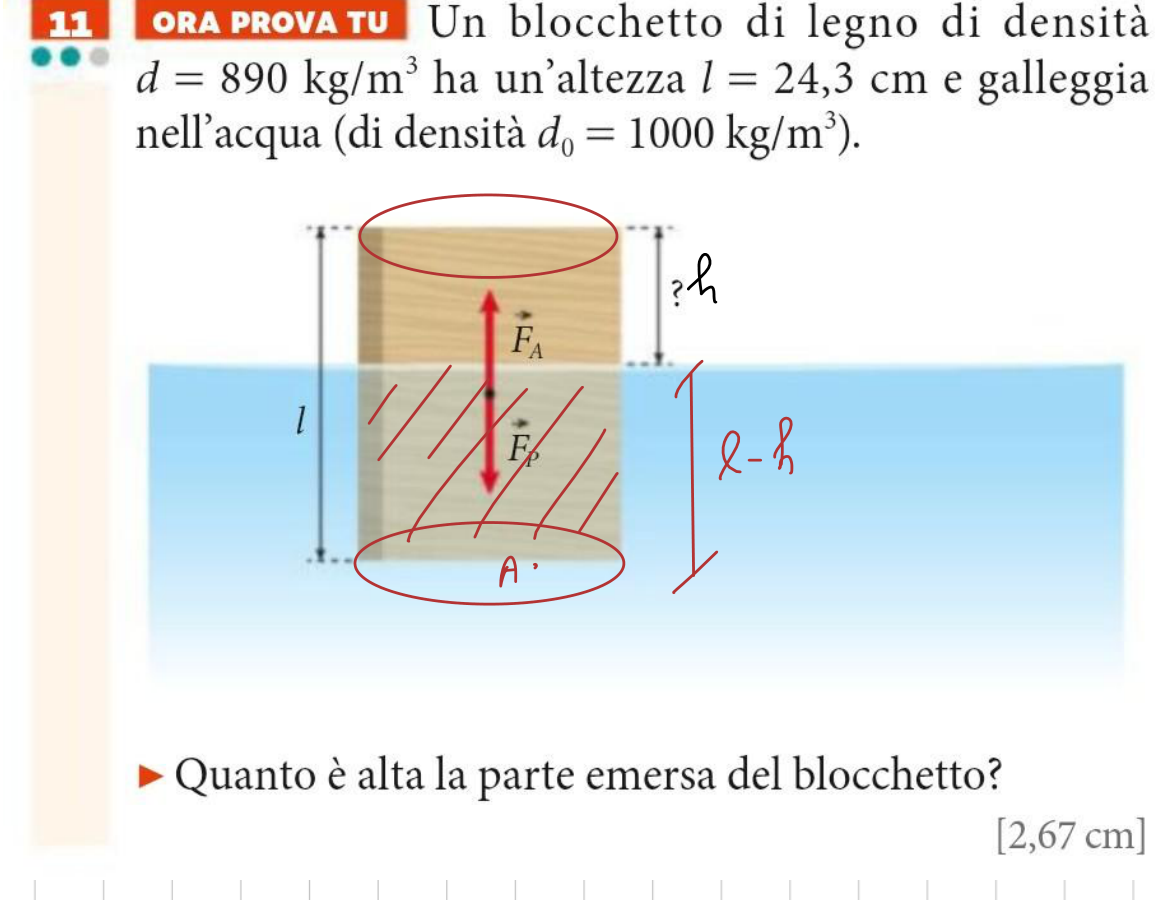
\includegraphics[width=0.72\linewidth]{immagini/es_11_galleggiamento.png}

\vspace{0.3cm}
\raggedright
\textbf{Dati:}
\begin{itemize}
  \item Densit\`a del blocchetto: $d_c = 890\,\text{kg/m}^3$;
  \item Altezza totale del blocchetto: $l = 24{,}3\,\text{cm} = 0{,}243\,\text{m}$;
  \item Densit\`a dell'acqua: $d_0 = 1000\,\text{kg/m}^3$.
\end{itemize}

\textbf{Risoluzione analitica:}\\
All'equilibrio di galleggiamento, la forza peso bilancia la spinta di Archimede:
\[
F_A = F_p \implies d_0 \cdot g \cdot V_{\text{imm}} = d_c \cdot g \cdot V_c
\]
Indicando con $A$ la sezione trasversale del cilindro, il volume immerso \`e $V_{\text{imm}} = A \cdot (l - h)$, mentre il volume complessivo \`e $V_c = A \cdot l$:
\[
d_0 \cdot g \cdot A (l - h) = d_c \cdot g \cdot A \cdot l \implies d_0 (l - h) = d_c \cdot l
\]
Esplicitando l'altezza emersa $h$:
\[
d_0 \cdot l - d_0 \cdot h = d_c \cdot l \implies \mathbf{h = l \left(1 - \frac{d_c}{d_0}\right)}
\]
\textbf{Calcolo numerico:}
\[
h = 0{,}243\,\text{m} \cdot \left(1 - \frac{890}{1000}\right) = 0{,}243\,\text{m} \cdot 0{,}110 = 0{,}02673\,\text{m} \approx \mathbf{2{,}67\,\text{cm}}
\]
La percentuale di volume emerso rispetto al totale \`e:
\[
\frac{h}{l} = 1 - \frac{d_c}{d_0} = 1 - 0{,}89 = 0{,}11 = \mathbf{11\%}
\]
\end{problema}

% ==============================================================================
% CAPITOLO 2
% ==============================================================================
\chapter{Dinamica dei Fluidi Ideali ed Equazione di Continuit\`a}

\section{Modello di Fluido Ideale e Portata Volumetrica}

Nello studio della dinamica dei fluidi si assume il modello di \textbf{fluido ideale}: incompressibile ($\rho = \text{cost}$), privo di viscosit\`a ($\eta = 0$), con moto stazionario ($\partial \vec{v}/\partial t = 0$) e moto irrotazionale.
La \textbf{portata volumetrica} $Q$ rappresenta il volume di fluido $\Delta V$ che attraversa una sezione di area $A$ nell'intervallo di tempo $\Delta t$:
\[
Q = \frac{\Delta V}{\Delta t} = \frac{A \cdot \Delta x}{\Delta t} = A \cdot v \quad \left[\frac{\text{m}^3}{\text{s}}\right]
\]

\begin{leggefisica}[Equazione di Continuit\`a]
In virt\`u della conservazione della massa, per un fluido incompressibile in regime stazionario la portata si conserva identica in ogni sezione del condotto:
\[
\mathbf{A_1 \cdot v_1 = A_2 \cdot v_2 = \text{costante}} \implies \mathbf{v_2 = v_1 \left(\frac{A_1}{A_2}\right)}
\]
\end{leggefisica}

\begin{problema}[Esercizio 18 -- Condotto a Sezione Variabile]
Un fluido ideale scorre in regime stazionario attraverso una conduttura orizzontale a sezione variabile. Nella prima sezione, di area $A_1 = 2{,}0\,\text{cm}^2 = 0{,}00020\,\text{m}^2$, la velocit\`a del fluido \`e $v_1 = 6{,}0 \cdot 10^{-2}\,\text{m/s}$. Successivamente il condotto si restringe a una seconda sezione di area $A_2 = 0{,}80\,\text{cm}^2 = 0{,}000080\,\text{m}^2$.
Determinare la portata volumetrica $q$ della condotta e la velocit\`a $v_2$ con cui il fluido transita nella seconda sezione.

\textbf{Risoluzione:}\\
La portata volumetrica nella prima sezione \`e:
\[
q = A_1 \cdot v_1 = (2{,}0 \cdot 10^{-4}\,\text{m}^2) \cdot (6{,}0 \cdot 10^{-2}\,\text{m/s}) = \mathbf{1{,}2 \cdot 10^{-5}\,\text{m}^3/\text{s}}
\]
Applicando l'equazione di continuit\`a $q_1 = q_2 \implies A_1 v_1 = A_2 v_2$:
\[
v_2 = \frac{q}{A_2} = \frac{1{,}2 \cdot 10^{-5}\,\text{m}^3/\text{s}}{8{,}0 \cdot 10^{-5}\,\text{m}^2} = \mathbf{0{,}15\,\text{m/s}}
\]
La velocit\`a aumenta in proporzione inversa al rapporto tra le sezioni: $A_1 / A_2 = 2{,}0 / 0{,}80 = 2{,}5 \implies v_2 = 2{,}5 \cdot v_1$.
\end{problema}

\begin{problema}[Esercizio 21 -- Portata e Velocit\`a Sanguigna nell'Aorta Umana]
\centering
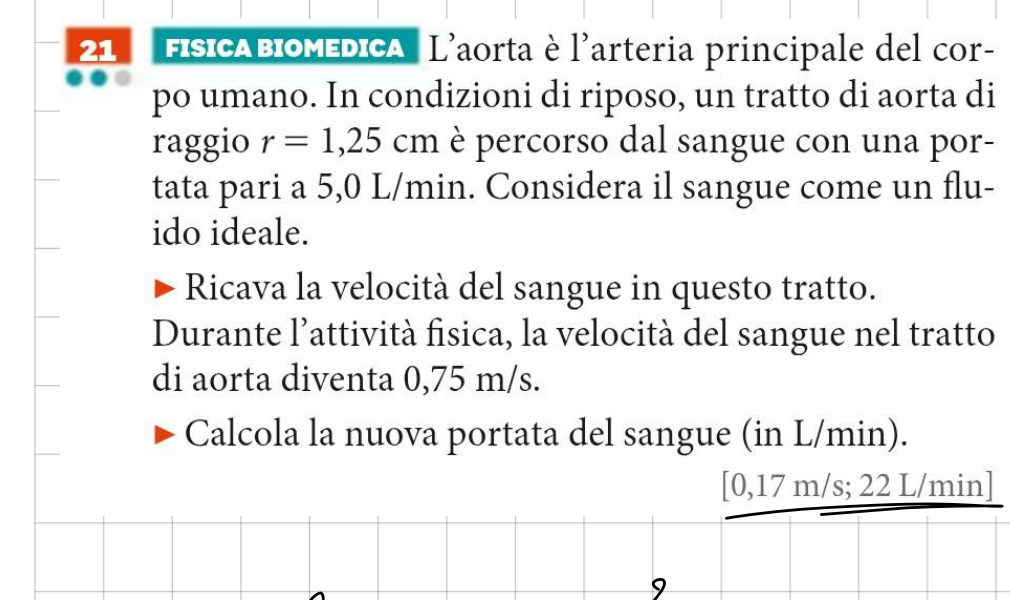
\includegraphics[width=0.72\linewidth]{immagini/es_21_aorta.png}

\vspace{0.3cm}
\raggedright
\textbf{Dati:}
\begin{itemize}
  \item Raggio dell'aorta a riposo: $r = 1{,}25\,\text{cm} = 1{,}25 \cdot 10^{-2}\,\text{m}$;
  \item Portata volumetrica a riposo: $q_1 = 5{,}0\,\text{L/min}$;
  \item Velocit\`a sanguigna durante attivit\`a fisica: $v_2 = 0{,}75\,\text{m/s}$.
\end{itemize}

\textbf{Risoluzione analitica:}\\
1. Convertiamo la portata in unit\`a fondamentali SI:
\[
q_1 = 5{,}0\,\frac{\text{L}}{\text{min}} = 5{,}0 \cdot \frac{10^{-3}\,\text{m}^3}{60\,\text{s}} \approx 8{,}33 \cdot 10^{-5}\,\text{m}^3/\text{s}
\]
L'area della sezione circolare dell'aorta \`e:
\[
A = \pi \cdot r^2 = \pi \cdot (1{,}25 \cdot 10^{-2}\,\text{m})^2 \approx 4{,}909 \cdot 10^{-4}\,\text{m}^2
\]
Ricaviamo la velocit\`a del sangue a riposo:
\[
v_1 = \frac{q_1}{A} = \frac{8{,}33 \cdot 10^{-5}\,\text{m}^3/\text{s}}{\pi \cdot (1{,}25 \cdot 10^{-2}\,\text{m})^2} \approx \mathbf{0{,}17\,\text{m/s}}
\]
2. Assumendo che il calibro dell'aorta $A$ rimanga invariato, la portata \`e direttamente proporzionale alla velocit\`a:
\[
\frac{q_1}{v_1} = \frac{q_2}{v_2} \implies \mathbf{q_2 = q_1 \cdot \frac{v_2}{v_1}}
\]
Sostituendo i valori:
\[
q_2 = 5{,}0\,\frac{\text{L}}{\text{min}} \cdot \frac{0{,}75\,\text{m/s}}{0{,}17\,\text{m/s}} \approx \mathbf{22\,\text{L/min}}
\]
Durante lo sforzo la portata cardiaca si moltiplica di oltre 4 volte per soddisfare l'aumentata richiesta aerobica dei tessuti.
\end{problema}

% ==============================================================================
% CAPITOLO 3
% ==============================================================================
\chapter{L'Equazione di Bernoulli, l'Effetto Venturi e Torricelli}

\section{Dimostrazione Rigorosa del Teorema di Bernoulli}

L'equazione di Bernoulli costituisce la formulazione del \textbf{teorema lavoro-energia cinetica} per un fluido ideale in regime stazionario.
Consideriamo un elemento di fluido di volume $\Delta V$ e massa $\Delta m = \rho \Delta V$ che si sposta da una sezione $A$ (a quota $y_A$ con pressione $p_A$ e velocit\`a $v_A$) a una sezione $B$ (a quota $y_B$ con pressione $p_B$ e velocit\`a $v_B$).

\textbf{1. Lavoro delle forze di pressione (forze non conservative):}\\
Il fluido a monte compie lavoro motore spingendo con forza $F_A = p_A S_A$, mentre il fluido a valle si oppone con forza resistente $F_B = p_B S_B$:
\[
W_{nc} = F_A \Delta x_A - F_B \Delta x_B = p_A S_A \Delta x_A - p_B S_B \Delta x_B = (p_A - p_B) \Delta V
\]
\textbf{2. Variazione di energia meccanica:}\\
L'energia cinetica e potenziale dell'elemento variano secondo:
\[
\Delta E_k = \frac{1}{2}\Delta m v_B^2 - \frac{1}{2}\Delta m v_A^2 = \frac{1}{2}\rho \Delta V (v_B^2 - v_A^2)
\]
\[
\Delta E_p = \Delta m g y_B - \Delta m g y_A = \rho \Delta V g (y_B - y_A)
\]
\textbf{3. Bilancio energetico $W_{nc} = \Delta E = \Delta E_k + \Delta E_p$:}\\
Uguagliando le espressioni e semplificando il volume comune $\Delta V$:
\[
(p_A - p_B)\Delta V = \rho \Delta V \left[ \frac{1}{2}(v_B^2 - v_A^2) + g(y_B - y_A) \right]
\]
Riorganizzando i termini tra monte e valle si giunge alla legge invariante:
\[
\mathbf{p_A + \frac{1}{2}\rho v_A^2 + \rho g y_A = p_B + \frac{1}{2}\rho v_B^2 + \rho g y_B = \text{costante}}
\]

\section{L'Effetto Venturi}

In una condotta orizzontale priva di dislivelli ($y_A = y_B = h$), l'equazione di Bernoulli si riduce a:
\[
\mathbf{p + \frac{1}{2}\rho v^2 = \text{costante}}
\]
Poich\'e la somma deve rimanere invariata, \textbf{se la velocit\`a aumenta nella strozzatura ($v_2 > v_1$), la pressione statica deve diminuire ($p_2 < p_1$)}.

\section{Il Teorema di Torricelli ed Efflusso da Serbatoio}

Per un serbatoio a pelo libero aperto all'atmosfera ($p_A = p_0$) con foro di uscita a profondit\`a $h$ ($p_B = p_0$), assumendo che la superficie libera sia vastissima rispetto all'orifizio ($A \gg B \implies v_A \approx 0$), Bernoulli porge:
\[
p_0 + \rho g h + 0 = p_0 + \frac{1}{2}\rho v_B^2 \implies \mathbf{v_B = \sqrt{2 \cdot g \cdot h}}
\]
La velocit\`a di efflusso coincide con quella di caduta libera da fermo da quota $h$.

\begin{problema}[Esercizio 53 -- Abbeveratoio con Tubo Inclinato e Moto Parabolico]
\centering
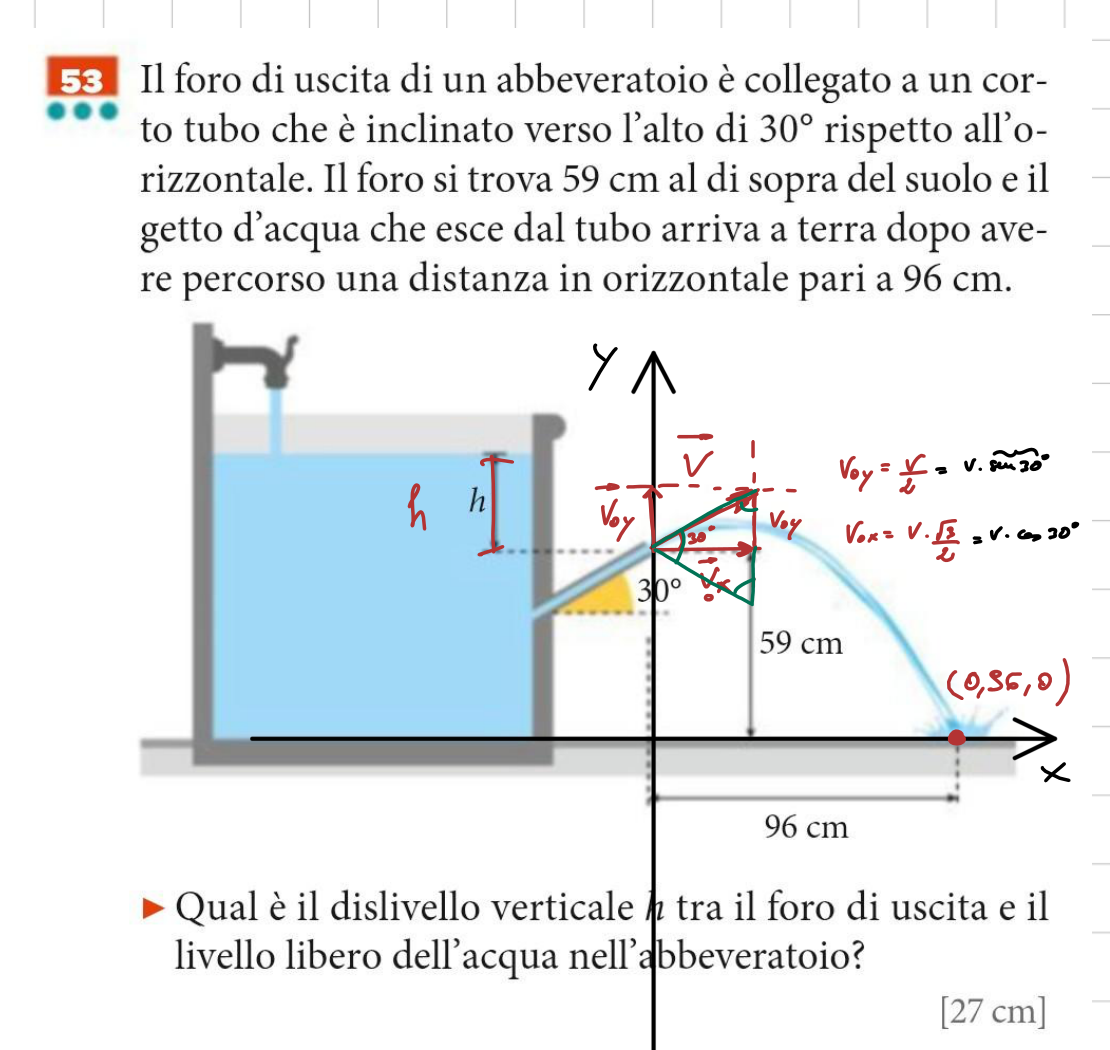
\includegraphics[width=0.72\linewidth]{immagini/es_53_abbeveratoio.png}

\vspace{0.3cm}
\raggedright
\textbf{Dati:}
\begin{itemize}
  \item Inclinazione del tubo rispetto all'orizzontale: $\theta = 30\,{^\circ}$;
  \item Quota del foro rispetto al suolo: $y_0 = 59\,\text{cm} = 0{,}59\,\text{m}$;
  \item Gittata orizzontale al suolo: $x = 96\,\text{cm} = 0{,}96\,\text{m}$;
  \item Dislivello $h$ tra pelo libero e foro: incognita.
\end{itemize}

\textbf{Risoluzione analitica:}\\
Il getto d'acqua fuoriesce con velocit\`a $v$ inclinata di $\theta = 30\,{^\circ}$. Le componenti della velocit\`a iniziale sono:
\[
v_{0x} = v \cos 30\,{^\circ} = v \frac{\sqrt{3}}{2}, \qquad v_{0y} = v \sin 30\,{^\circ} = \frac{v}{2}
\]
L'equazione oraria della traiettoria nel piano cartesiano $(x, y)$ con origine alla base del foro \`e:
\[
x(t) = v_{0x} \cdot t \implies t = \frac{x}{v_{0x}}
\]
\[
y(t) = y_0 + v_{0y} t - \frac{1}{2}g t^2 = y_0 + x \tan 30\,{^\circ} - \frac{g x^2}{2 v_{0x}^2}
\]
Imponendo l'impatto col suolo a $y = 0$ per $x = 0{,}96\,\text{m}$:
\[
0 = y_0 + x \frac{\sin 30\,{^\circ}}{\cos 30\,{^\circ}} - \frac{g x^2}{2 \left(v \frac{\sqrt{3}}{2}\right)^2} = y_0 + \frac{x}{\sqrt{3}} - \frac{2 g x^2}{3 v^2}
\]
Esplicitando il termine cinetico $1/v^2$:
\[
\frac{2 g x^2}{3 v^2} = y_0 + \frac{x}{\sqrt{3}} \implies \frac{1}{v^2} = \frac{3}{2 x^2} \left( \frac{y_0}{g} + \frac{x}{\sqrt{3} g} \right)
\]
Sostituendo i valori numerici:
\[
\frac{1}{v^2} = \frac{3}{2 \cdot (0{,}96)^2} \left( \frac{0{,}59}{9{,}81} + \frac{0{,}96}{1{,}732 \cdot 9{,}81} \right) \approx 1{,}6276 \cdot (0{,}06014 + 0{,}05650) \approx 0{,}1898\,\text{s}^2/\text{m}^2
\]
\[
v = \sqrt{\frac{1}{0{,}1898}} \approx \mathbf{2{,}30\,\text{m/s}}
\]
Applicando il teorema di Torricelli $v = \sqrt{2gh}$, ricaviamo il dislivello $h$:
\[
h = \frac{v^2}{2g} = \frac{(2{,}30\,\text{m/s})^2}{2 \cdot 9{,}81\,\text{m/s}^2} \approx \frac{5{,}29}{19{,}62} \approx 0{,}2696\,\text{m} \approx \mathbf{27\,\text{cm}}
\]
\end{problema}

\begin{problema}[Esercizio 4 -- Serbatoio Idraulico con Tappo Circolare e Zampillo]
\centering
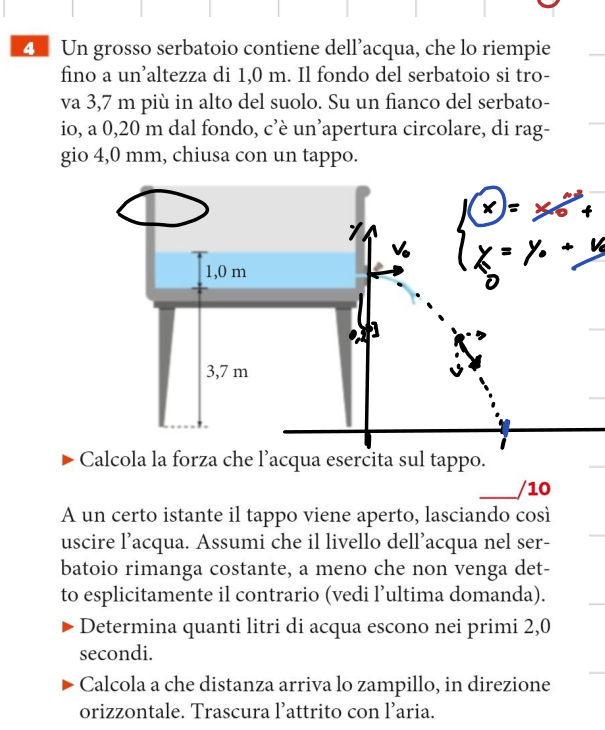
\includegraphics[width=0.65\linewidth]{immagini/es_04_serbatoio.png}

\vspace{0.3cm}
\raggedright
\textbf{Dati:}
\begin{itemize}
  \item Altezza dell'acqua nel serbatoio: $H_1 = 1{,}0\,\text{m}$;
  \item Fondo serbatoio a quota $3{,}7\,\text{m}$ dal suolo;
  \item Apertura circolare a $0{,}20\,\text{m}$ dal fondo, raggio $r = 4{,}0\,\text{mm} = 4{,}0 \cdot 10^{-3}\,\text{m}$.
\end{itemize}

\textbf{Risoluzione:}\\
1. \textbf{Forza idrostatica sul tappo:}\\
La profondit\`a del foro rispetto al pelo libero \`e $h = 1{,}0\,\text{m} - 0{,}20\,\text{m} = 0{,}80\,\text{m}$. La pressione relativa esercitata dall'acqua \`e $p_{\text{idr}} = \rho g h = 1000 \cdot 9{,}81 \cdot 0{,}80 = 7848\,\text{Pa}$. L'area del foro \`e $S = \pi r^2 = \pi (4{,}0 \cdot 10^{-3})^2 \approx 5{,}03 \cdot 10^{-5}\,\text{m}^2$.
\[
F = p_{\text{idr}} \cdot S = 7848\,\text{Pa} \cdot 5{,}03 \cdot 10^{-5}\,\text{m}^2 \approx \mathbf{0{,}39\,\text{N}}
\]
2. \textbf{Volume erogato nei primi 2,0 secondi:}\\
Velocit\`a di efflusso orizzontale di Torricelli: $v = \sqrt{2gh} = \sqrt{2 \cdot 9{,}81 \cdot 0{,}80} \approx 3{,}96\,\text{m/s}$.
Portata volumetrica: $Q = S \cdot v = (5{,}03 \cdot 10^{-5}) \cdot 3{,}96 \approx 1{,}99 \cdot 10^{-4}\,\text{m}^3/\text{s} \approx 0{,}199\,\text{L/s}$.
Nei primi $\Delta t = 2{,}0\,\text{s}$:
\[
V = Q \cdot \Delta t = 0{,}199\,\text{L/s} \cdot 2{,}0\,\text{s} \approx \mathbf{0{,}40\,\text{L}}
\]
3. \textbf{Gittata orizzontale dello zampillo:}\\
La quota del foro dal suolo \`e $y_0 = 3{,}7\,\text{m} + 0{,}20\,\text{m} = 3{,}9\,\text{m}$. Il tempo di caduta libera \`e:
\[
t_c = \sqrt{\frac{2 y_0}{g}} = \sqrt{\frac{2 \cdot 3{,}9\,\text{m}}{9{,}81\,\text{m/s}^2}} \approx 0{,}89\,\text{s}
\]
La gittata orizzontale \`e:
\[
x = v \cdot t_c = 3{,}96\,\text{m/s} \cdot 0{,}89\,\text{s} \approx \mathbf{3{,}5\,\text{m}}
\]
4. \textbf{Tempo per abbassare il livello di $s = 0{,}01\,\text{m}$ (1 cm):}\\
Per un serbatoio con area superficiale $A_1 = 8{,}2\,\text{m}^2$, la velocit\`a di discesa \`e $v_1 = Q / A_1 = (1{,}99 \cdot 10^{-4})/8{,}2 \approx 0{,}24 \cdot 10^{-4}\,\text{m/s}$. Il tempo richiesto \`e:
\[
t = \frac{s}{v_1} = \frac{0{,}01\,\text{m}}{0{,}24 \cdot 10^{-4}\,\text{m/s}} \approx 411{,}8\,\text{s} \approx \mathbf{4{,}1 \cdot 10^2\,\text{s}}
\]
\end{problema}

\begin{problema}[Esercizio 45 -- Foro di Deflusso in Diga di Irrigazione]
\centering
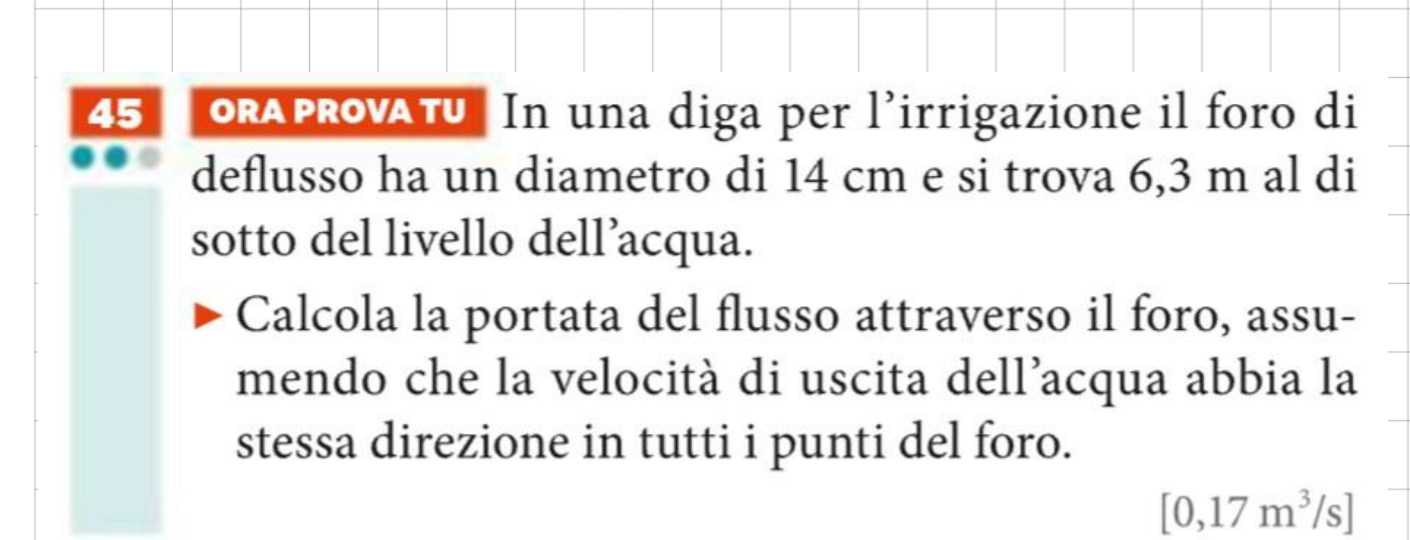
\includegraphics[width=0.72\linewidth]{immagini/es_45_diga.png}

\vspace{0.3cm}
\raggedright
\textbf{Dati:}
\begin{itemize}
  \item Diametro del foro: $d = 14\,\text{cm} = 0{,}14\,\text{m}$;
  \item Profondit\`a al di sotto del pelo libero: $h_A = 6{,}3\,\text{m}$.
\end{itemize}

\textbf{Risoluzione:}\\
Dall'equazione di Bernoulli, la velocit\`a di efflusso al foro \`e governata dal teorema di Torricelli:
\[
v_B = \sqrt{2 \cdot g \cdot h_A} = \sqrt{2 \cdot 9{,}81\,\text{m/s}^2 \cdot 6{,}3\,\text{m}} \approx \sqrt{123{,}6} \approx 11{,}1\,\text{m/s}
\]
L'area della sezione circolare del foro \`e:
\[
A = \frac{\pi \cdot d^2}{4} = \frac{\pi \cdot (0{,}14\,\text{m})^2}{4} \approx 0{,}01539\,\text{m}^2
\]
La portata volumetrica $q$ \`e data dal prodotto:
\[
q = A \cdot v_B = \frac{\pi \cdot d^2}{4} \sqrt{2 g h_A} = 0{,}01539\,\text{m}^2 \cdot 11{,}1\,\text{m/s} \approx \mathbf{0{,}17\,\text{m}^3/\text{s}}
\]
\end{problema}

\begin{problema}[Esercizio 79 -- Condotto con Pompa ed Erogatore Finale]
\centering
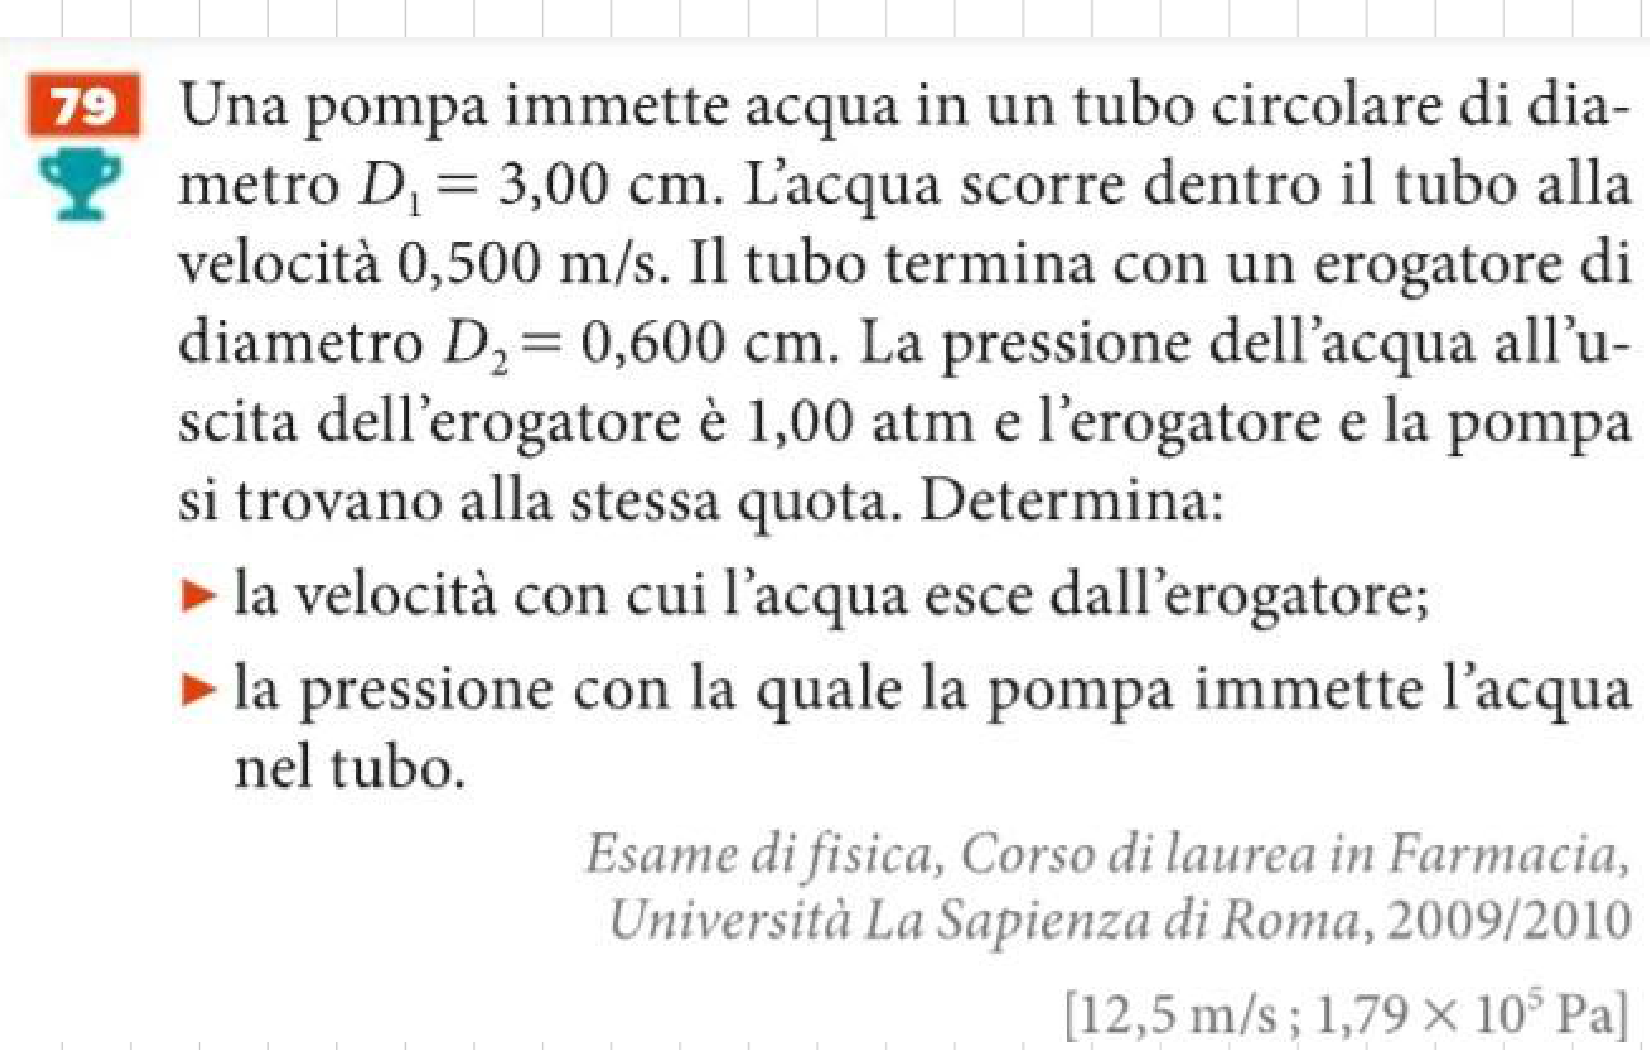
\includegraphics[width=0.75\linewidth]{immagini/es_79_pompa.png}

\vspace{0.3cm}
\raggedright
\textbf{Dati:}
\begin{itemize}
  \item Diametro del tubo: $D_1 = 3{,}00\,\text{cm} = 0{,}030\,\text{m}$;
  \item Velocit\`a nel tubo: $v_1 = 0{,}500\,\text{m/s}$;
  \item Diametro dell'erogatore: $D_2 = 0{,}600\,\text{cm} = 0{,}0060\,\text{m}$;
  \item Pressione atmosferica all'uscita: $p_2 = 1{,}00\,\text{atm} = 1{,}013 \cdot 10^5\,\text{Pa}$;
  \item Condotto orizzontale a quota costante ($y_1 = y_2$).
\end{itemize}

\textbf{Risoluzione:}\\
1. \textbf{Velocit\`a all'uscita dell'erogatore ($v_2$):}\\
Dall'equazione di continuit\`a $A_1 v_1 = A_2 v_2$:
\[
v_2 = v_1 \left(\frac{A_1}{A_2}\right) = v_1 \left(\frac{D_1}{D_2}\right)^2 = 0{,}500\,\text{m/s} \cdot \left(\frac{0{,}030}{0{,}0060}\right)^2 = 0{,}500 \cdot 5^2 = 0{,}500 \cdot 25 = \mathbf{12{,}5\,\text{m/s}}
\]
2. \textbf{Pressione immessa dalla pompa ($p_1$):}\\
Applicando l'equazione di Bernoulli orizzontale:
\[
p_1 + \frac{1}{2}\rho v_1^2 = p_2 + \frac{1}{2}\rho v_2^2 \implies \mathbf{p_1 = p_2 + \frac{1}{2}\rho (v_2^2 - v_1^2)}
\]
Calcoliamo la variazione di pressione dinamica per l'acqua ($\rho = 1000\,\text{kg/m}^3$):
\[
\Delta p_{\text{din}} = \frac{1}{2} \cdot 1000 \cdot \left[ (12{,}5)^2 - (0{,}5)^2 \right] = 500 \cdot (156{,}25 - 0{,}25) = 500 \cdot 156 = 78\,000\,\text{Pa} = 0{,}78 \cdot 10^5\,\text{Pa}
\]
Sommando alla pressione atmosferica di uscita $p_2$:
\[
p_1 = 1{,}013 \cdot 10^5\,\text{Pa} + 0{,}78 \cdot 10^5\,\text{Pa} \approx \mathbf{1{,}79 \cdot 10^5\,\text{Pa}}
\]
\end{problema}

% ==============================================================================
% CAPITOLO 4
% ==============================================================================
\chapter{Fluidi Reali e Viscosit\`a: Legge di Poiseuille}

\section{Attrito Viscoso e Profilo Parabolico}

Nei fluidi reali le forze di attrito intermolecolare generano resistenza allo scorrimento, quantificata dalla viscosit\`a dinamica $\eta$ [$\text{Pa}\cdot\text{s}$]. Per la condizione di non scivolamento alle pareti ($v = 0$), la velocit\`a presenta un \textbf{profilo laminare parabolico}:
\[
v(r) = v_{\text{max}} \left(1 - \frac{r^2}{R^2}\right)
\]

\begin{leggefisica}[Legge di Poiseuille]
La portata volumetrica $Q$ di un fluido viscoso in moto laminare in un condotto cilindrico di raggio $R$ e lunghezza $L$ sotto un gradiente di pressione $\Delta p$ \`e data da:
\[
\mathbf{Q = \frac{\pi \cdot R^4 \cdot \Delta p}{8 \cdot \eta \cdot L}}
\]
\end{leggefisica}

La dipendenza da $R^4$ rende la portata sensibilmente dipendente dal raggio: una riduzione del calibro vascolare di appena il $16\%$ dimezza la portata sanguigna a parit\`a di pressione.

% ==============================================================================
% PARTE II: TERMODINAMICA DEI GAS
% ==============================================================================

\chapter{Sistemi Termodinamici ed Equilibrio Termico: Il Principio Zero}

\section{Definizione di Temperatura e Sistemi Termodinamici}

In termodinamica, due corpi posti a contatto termico hanno la \textbf{stessa temperatura} se e solo se si trovano in \textbf{equilibrio termico} tra loro (ovvero non vi \`e alcun flusso netto di calore tra essi). Viceversa, se due corpi sono in equilibrio termico, essi possiedono identica temperatura.

\begin{definizione}[Sistema Termodinamico e Ambiente]
Un \textbf{sistema termodinamico} \`e una porzione definita di materia separata dal resto dell'universo (denominato \textbf{ambiente}) mediante una superficie di confine reale o ideale.
\end{definizione}

La materia gassosa racchiusa in un recipiente costituisce il prototipo fondamentale di sistema termodinamico. I sistemi si classificano in tre categorie essenziali:
\begin{enumerate}
  \item \textbf{Sistema Aperto:} pu\`o scambiare con l'ambiente sia materia sia energia (ad esempio una pentola d'acqua in ebollizione priva di coperchio);
  \item \textbf{Sistema Chiuso:} pu\`o scambiare con l'ambiente energia (sotto forma di calore o lavoro), ma non materia (ad esempio un cilindro sigillato dotato di pistone mobile);
  \item \textbf{Sistema Isolato:} non pu\`o scambiare con l'ambiente n\'e materia n\'e alcuna forma di energia (ad esempio un termos ideale perfettamente coibentato).
\end{enumerate}

\section{Il Principio Zero della Termodinamica}

\begin{leggefisica}[Principio Zero della Termodinamica]
Se un corpo $A$ si trova in equilibrio termico con un corpo $B$, e il corpo $B$ si trova a sua volta in equilibrio termico con un terzo corpo $C$, allora i corpi $A$ e $C$ sono necessariamente in equilibrio termico tra loro:
\[
A \sim B \quad \land \quad B \sim C \implies A \sim C
\]
\end{leggefisica}

\begin{commento}[Significato Operativo del Principio Zero e Costruzione del Termometro]
Il Principio Zero garantisce la propriet\`a transitiva dell'equilibrio termico. Esso fornisce la giustificazione teorica essenziale che consente di definire la temperatura come propriet\`a intrinseca di stato e rende possibile l'esistenza dei \textbf{termometri}: impiegando il corpo $B$ come strumento di misura (termometro a mercurio o digitale), possiamo confrontare le temperature di due sistemi fisici indipendenti $A$ e $C$ senza doverli porre a diretto contatto reciproco.
\end{commento}

% ==============================================================================
% CAPITOLO 6
% ==============================================================================
\chapter{La Misura della Quantit\`a di Sostanza: Mole e Massa Molare}

\section{Atomi, Molecole e Unit\`a di Massa Atomica}

Ogni sostanza pura \`e costituita da particelle elementari caratteristiche (atomi o molecole). Ad esempio, la molecola d'acqua $\text{H}_2\text{O}$ \`e formata da due atomi di idrogeno legati a un atomo di ossigeno. Ciascun atomo possiede un nucleo contenente protoni ($p$) e neutroni ($n$) circondato da elettroni. Per l'ossigeno il numero atomico \`e $Z = 8$ e il numero di massa \`e $A \approx 16{,}00$.

Poich\'e le masse atomiche sono minuscole, si definisce l'\textbf{unit\`a di massa atomica unificata} ($u$):
\[
\mathbf{1\,\text{u} \approx 1{,}6605 \cdot 10^{-27}\,\text{kg}}
\]
La massa molecolare della sostanza \`e la somma delle masse atomiche dei singoli costituenti. Per l'acqua:
\[
m_{\text{H}_2\text{O}} = m_{\text{O}} + 2 \cdot m_{\text{H}} = 16{,}00\,\text{u} + 2 \cdot 1{,}008\,\text{u} = \mathbf{18{,}02\,\text{u}}
\]

\section{La Mole e la Costante di Avogadro}

\begin{leggefisica}[Definizione di Mole e Costante di Avogadro]
La \textbf{mole} (simbolo $\text{mol}$) \`e la quantit\`a di sostanza che contiene un numero di entit\`a elementari (atomi o molecole) esattamente pari alla \textbf{Costante di Avogadro} $N_A$:
\[
\mathbf{N_A = 6{,}022 \cdot 10^{23}\,\text{mol}^{-1}}
\]
Il numero totale di particelle $N$ \`e collegato al numero di moli $n$ dalla relazione:
\[
\mathbf{N = n \cdot N_A} \iff \mathbf{n = \frac{N}{N_A}}
\]
\end{leggefisica}

\section{La Massa Molare}

La \textbf{massa molare} $M$ di una sostanza \`e definita come il rapporto tra la massa $m$ in grammi di un campione macroscopico e il numero di moli $n$ che esso contiene:
\[
\mathbf{M = \frac{m}{n}} \quad \left[\frac{\text{g}}{\text{mol}}\right] \iff \mathbf{m = n \cdot M}
\]
Numericamente, la massa molare espressa in $\text{g/mol}$ coincide con la massa atomica o molecolare espressa in unit\`a di massa atomica ($u$).

\begin{problema}[Esercizio 33 -- Moli Contenute in un Campione di Glucosio]
\centering
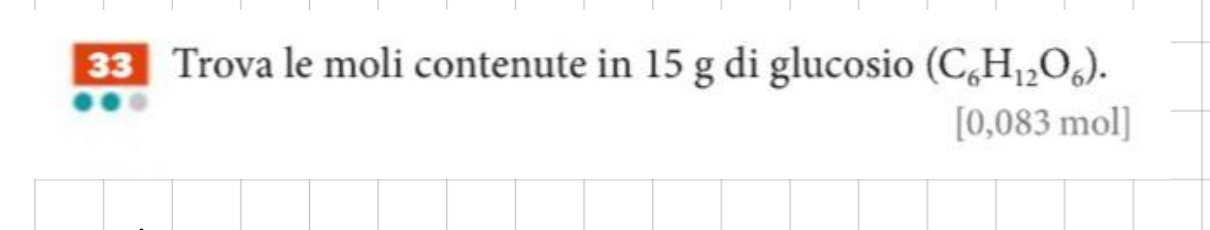
\includegraphics[width=0.72\linewidth]{immagini/es_33_glucosio.png}

\vspace{0.3cm}
\raggedright
\textbf{Dati:}
\begin{itemize}
  \item Massa del campione: $m = 15\,\text{g}$;
  \item Formula molecolare del glucosio: $\text{C}_6\text{H}_{12}\text{O}_6$.
\end{itemize}

\textbf{Risoluzione:}\\
Determiniamo la massa molare $M$ del glucosio sommando i contributi atomici di carbonio ($12\,\text{g/mol}$), idrogeno ($1{,}0\,\text{g/mol}$) e ossigeno ($16\,\text{g/mol}$):
\[
M_{\text{C}_6\text{H}_{12}\text{O}_6} = 6 \cdot m_{\text{C}} + 12 \cdot m_{\text{H}} + 6 \cdot m_{\text{O}} = (6 \cdot 12) + (12 \cdot 1) + (6 \cdot 16) = 72 + 12 + 96 = \mathbf{180\,\text{g/mol}}
\]
Il numero di moli $n$ contenute nei $15\,\text{g}$ \`e:
\[
n = \frac{m}{M} = \frac{15\,\text{g}}{180\,\text{g/mol}} \approx \mathbf{0{,}083\,\text{mol}}
\]
\end{problema}

\begin{problema}[Esercizi 26 e 27 -- Massa Atomica e Moli del Neon]
\centering
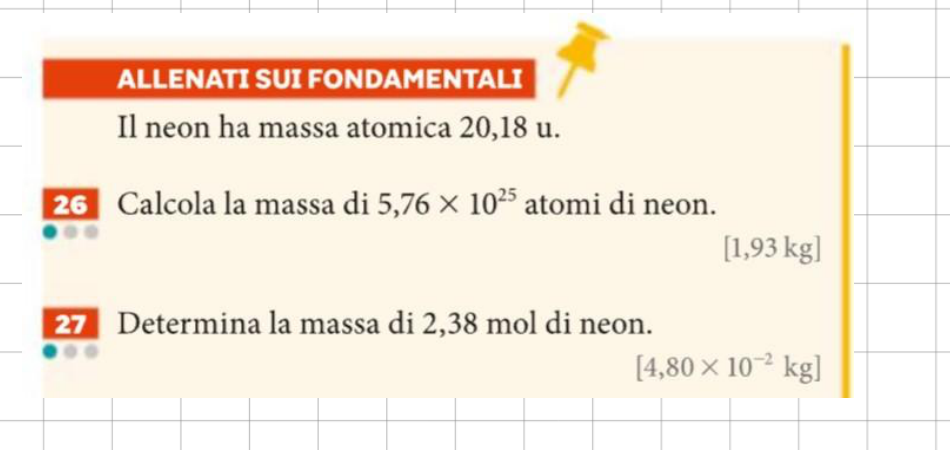
\includegraphics[width=0.70\linewidth]{immagini/es_26_neon.png}

\vspace{0.3cm}
\raggedright
\textbf{Dati:}
\begin{itemize}
  \item Massa atomica del neon: $M_{\text{Ne}} = 20{,}18\,\text{u} \implies M = 20{,}18\,\text{g/mol}$;
  \item Esercizio 26: $N = 5{,}76 \cdot 10^{25}$ atomi di neon;
  \item Esercizio 27: $n = 2{,}38\,\text{mol}$ di neon.
\end{itemize}

\textbf{Risoluzione Esercizio 26:}\\
Ricaviamo il numero di moli corrispondente agli atomi assegnati:
\[
n = \frac{N}{N_A} = \frac{5{,}76 \cdot 10^{25}}{6{,}022 \cdot 10^{23}\,\text{mol}^{-1}} \approx 95{,}65\,\text{mol}
\]
La massa complessiva in grammi e chilogrammi \`e:
\[
m = n \cdot M = 95{,}65\,\text{mol} \cdot 20{,}18\,\frac{\text{g}}{\text{mol}} \approx 1930\,\text{g} \approx \mathbf{1{,}93\,\text{kg}}
\]

\textbf{Risoluzione Esercizio 27:}\\
Per $n = 2{,}38\,\text{mol}$ di neon:
\[
m = n \cdot M = 2{,}38\,\text{mol} \cdot 20{,}18\,\frac{\text{g}}{\text{mol}} = 48{,}03\,\text{g} = \mathbf{4{,}80 \cdot 10^{-2}\,\text{kg}}
\]
\end{problema}

% ==============================================================================
% CAPITOLO 7
% ==============================================================================
\chapter{Le Leggi Sperimentali dei Gas Perfetti nel Piano di Clapeyron}

\section{La Legge di Boyle (Trasformazione Isoterma)}

Consideriamo un gas perfetto racchiuso in un cilindro con pistone a tenuta mobile, immerso in un capiente bagno termico a temperatura costante $T$. Variando il carico di pesetti sul pistone, la pressione $p = p_{\text{atm}} + F_p / A$ varia lentamente in condizioni di equilibrio termico.

\begin{leggefisica}[Legge di Boyle]
A temperatura costante ($T = \text{cost}$), la pressione $p$ e il volume $V$ di una massa determinata di gas sono inversamente proporzionali:
\[
\mathbf{p \cdot V = \text{costante}} \iff \mathbf{p_1 \cdot V_1 = p_2 \cdot V_2}
\]
Nel piano di Clapeyron $(V, p)$, la trasformazione isoterma \`e rappresentata da un \textbf{ramo di iperbole equilatera}.
\end{leggefisica}

\begin{figure}[H]
\centering
\begin{tikzpicture}[scale=0.92, >=stealth]
  \draw[->, thick, primaryBlue] (0, 0) -- (7.2, 0) node[below right, font=\small\sffamily] {$V \, [\text{m}^3]$};
  \draw[->, thick, primaryBlue] (0, 0) -- (0, 5.4) node[above left, font=\small\sffamily] {$p \, [\text{Pa}]$};
  \node[below left, primaryBlue] at (0, 0) {$O$};
  
  % Asintoti cartesiani
  \node[above, gray!70, font=\scriptsize] at (0.3, 4.9) {Asintoto $V = 0$};
  \node[right, gray!70, font=\scriptsize] at (5.8, 0.2) {Asintoto $p = 0$};

  % Famiglia di rami di iperbole equilatera (isoterme)
  \draw[thick, accentRed!50, domain=0.7:6.4, samples=100] plot (\x, {2.0/\x}) node[right, font=\footnotesize] {Isoterma $T_1$};
  \draw[very thick, accentRed, domain=0.9:6.4, samples=100] plot (\x, {3.6/\x}) node[right, font=\footnotesize\bfseries] {Isoterma $T_2 > T_1$ ($p \cdot V = \text{cost}$)};
  \draw[thick, accentRed!80!black, domain=1.3:6.4, samples=100] plot (\x, {5.6/\x}) node[right, font=\footnotesize] {Isoterma $T_3 > T_2$};

  % Punti notevoli sull'isoterma T2
  \draw[dashed, gray] (1.2, 0) node[below, font=\footnotesize] {$V_1$} -- (1.2, 3.0) -- (0, 3.0) node[left, font=\footnotesize] {$p_1$};
  \draw[dashed, gray] (4.0, 0) node[below, font=\footnotesize] {$V_2$} -- (4.0, 0.9) -- (0, 0.9) node[left, font=\footnotesize] {$p_2$};
  \fill[primaryBlue] (1.2, 3.0) circle (2.5pt);
  \node[above right, font=\footnotesize\bfseries, fill=white, fill opacity=0.9, text opacity=1, inner sep=1.5pt] at (1.2, 3.0) {$A(V_1, p_1)$};
  \fill[primaryBlue] (4.0, 0.9) circle (2.5pt);
  \node[above right, font=\footnotesize\bfseries, fill=white, fill opacity=0.9, text opacity=1, inner sep=1.5pt] at (4.0, 0.9) {$B(V_2, p_2)$};
  
  % Freccia di espansione da A verso B
  \draw[-{Latex[length=3mm]}, very thick, accentAmber] (2.2, 1.636) -- (2.8, 1.285) node[midway, above right, font=\scriptsize\bfseries, fill=white, inner sep=1pt] {Espansione};
\end{tikzpicture}
\caption{Trasformazione isoterma di Boyle nel piano di Clapeyron: le curve a temperatura costante costituiscono una famiglia di rami di iperbole equilatera aventi per asintoti gli assi cartesiani ($V = 0$ e $p = 0$). All'aumentare della temperatura ($T_1 < T_2 < T_3$), i rami iperbolici si allontanano progressivamente dall'origine degli assi ($p \cdot V = n R T$).}
\label{fig:boyle_clapeyron}
\end{figure}

\section{La Prima Legge di Gay-Lussac (Trasformazione Isobara)}

Lasciando il pistone libero di muoversi sotto un carico di peso costante, la pressione del gas rimane fissa ($p = \text{cost}$). Riscaldando il contenitore, il gas si espande linearmente con la temperatura centigrada $t$:
\[
\mathbf{V(t) = V_0 (1 + \alpha \cdot t)}
\]
dove $V_0$ \`e il volume a $0\,{^\circ}\text{C}$ e $\alpha = \frac{1}{273{,}15\,{^\circ}\text{C}} \approx 0{,}00366\,{^\circ}\text{C}^{-1}$ \`e il \textbf{coefficiente di dilatazione volumica dei gas}, universale per tutti i gas rarefatti.
Nel piano di Clapeyron, l'isobara \`e un \textbf{segmento orizzontale}.
Nel grafico $V - t$, estrapolando la retta a volume nullo ($V = 0$):
\[
1 + \alpha t = 0 \implies t = -\frac{1}{\alpha} = \mathbf{-273{,}15\,{^\circ}\text{C}}
\]
Tale temperatura limite rappresenta lo \textbf{Zero Assoluto} della materia ($0\,\text{K}$).

\section{La Seconda Legge di Gay-Lussac (Trasformazione Isocora)}

Racchiudendo il gas in un contenitore rigido ermetico a volume costante ($V = \text{cost}$), la pressione aumenta linearmente all'aumentare della temperatura:
\[
\mathbf{p(t) = p_0 (1 + \alpha \cdot t)}
\]
Nel piano di Clapeyron, l'isocora \`e rappresentata da un \textbf{segmento verticale}.

\section{La Scala Assoluta Kelvin e la Forma Diretta delle Leggi}

Introducendo la \textbf{temperatura assoluta Kelvin} $T = t + 273{,}15\,\text{K}$, le leggi di Gay-Lussac assumono una forma lineare pura di diretta proporzionalit\`a:
\begin{itemize}
  \item \textbf{Prima Legge di Gay-Lussac (Isobara, $p = \text{cost}$):}
  \[
  \mathbf{\frac{V}{T} = \text{costante}} \iff \mathbf{\frac{V_1}{T_1} = \frac{V_2}{T_2}}
  \]
  \item \textbf{Seconda Legge di Gay-Lussac (Isocora, $V = \text{cost}$):}
  \[
  \mathbf{\frac{p}{T} = \text{costante}} \iff \mathbf{\frac{p_1}{T_1} = \frac{p_2}{T_2}}
  \]
\end{itemize}

\begin{approfondimento}[Ha senso raddoppiare la temperatura in gradi Celsius? Considerazioni fisiche e scale di misura]
\textbf{Risposta sintetica:} Dal punto di vista fisico e termodinamico, \textbf{no, non ha alcun senso}.

La scala Celsius \`e una \textbf{scala a intervalli} (o affinemente traslata) e non una \textbf{scala di rapporti}. Il suo valore zero ($0\,{^\circ}\text{C}$) \`e un riferimento puramente convenzionale (il punto di fusione del ghiaccio a pressione atmosferica standard) e non corrisponde affatto all'assenza di agitazione termica o moto molecolare a livello microscopico.

\subsection*{Le contraddizioni logiche e i paradossi fisici}
L'applicazione di operazioni moltiplicative a grandezze definite su scale prive di uno zero assoluto conduce immediatamente a insanabili paradossi logico-fisici:
\begin{itemize}[leftmargin=*, nosep]
  \item \textbf{Il paradosso dello zero:} Moltiplicare per due una temperatura di $0\,{^\circ}\text{C}$ restituirebbe ancora $0\,{^\circ}\text{C}$:
  \[
  2 \times 0\,{^\circ}\text{C} = 0\,{^\circ}\text{C}
  \]
  Ci\`o implicherebbe che l'energia cinetica interna del sistema resti perfettamente invariata, rendendo il ``raddoppio'' del tutto fittizio e nullo.
  \item \textbf{Il paradosso dei valori negativi:} Raddoppiare una temperatura negativa come $-10\,{^\circ}\text{C}$ porterebbe algebricamente a $-20\,{^\circ}\text{C}$. Tuttavia, uno stato a $-20\,{^\circ}\text{C}$ descrive un livello energetico inferiore (pi\`u freddo) rispetto a $-10\,{^\circ}\text{C}$, ribaltando e snaturando il significato fisico dell'operazione.
  \item \textbf{Inconsistenza energetica reale:} Passare da $10\,{^\circ}\text{C}$ a $20\,{^\circ}\text{C}$ non raddoppia affatto l'energia cinetica media molecolare. In unit\`a termodinamiche assolute:
  \[
  10\,{^\circ}\text{C} = 283{,}15\text{ K}, \quad 20\,{^\circ}\text{C} = 293{,}15\text{ K}
  \]
  Il rapporto effettivo tra le temperature assolute \`e:
  \[
  \frac{293{,}15}{283{,}15} \approx 1{,}0353 \implies +3{,}53\%
  \]
  L'incremento energetico reale \`e di appena il $3{,}5\%$, ben lontano dal $+100\%$ atteso da un vero raddoppio.
\end{itemize}

\subsection*{La prospettiva termodinamica corretta e la costante di Boltzmann}
La temperatura termodinamica rigorosa \`e una grandezza direttamente legata all'energia cinetica traslazionale media delle particelle che compongono la materia (per un gas ideale monoatomico):
\[
\langle E_k \rangle = \frac{3}{2} k_B T
\]
dove $k_B \approx 1{,}38 \times 10^{-23}\,\text{J/K}$ \`e la costante di Boltzmann e $T$ \`e la temperatura espressa nella scala assoluta dei \textbf{Kelvin} ($\text{K}$), il cui zero ($0\text{ K} = -273{,}15\,{^\circ}\text{C}$) corrisponde al limite asintotico di minima agitazione termica possibile.

\subsection*{Attenzione fondamentale negli esercizi: il tranello del ``raddoppio''}
\textbf{Avvertenza metodologica cruciale per compiti e verifiche:} Negli esercizi sui gas perfetti (trasformazioni isobare come nel successivo Esercizio 49, isocore o politropiche) si incontra spessissimo la formulazione:
\begin{center}
\textit{\textbf{<<La temperatura del gas raddoppia...>>}} \quad oppure \quad \textit{\textbf{<<Calcola a quale temperatura il volume raddoppia>>}}
\end{center}
\textbf{Bisogna prestare la massima attenzione all'unit\`a di misura!} Quando il testo di un problema afferma che la temperatura raddoppia, l'operazione moltiplicativa ($T_2 = 2 T_1$) deve essere applicata \textbf{tassativamente e unicamente alla temperatura assoluta in Kelvin ($T$)}, mai e poi mai ai gradi Celsius ($t$).

\textbf{Esempio pratico di calcolo corretto:}\\
Se un gas si trova inizialmente alla temperatura ambiente di $t_1 = 20\,{^\circ}\text{C}$, per \textbf{raddoppiare termodinamicamente la sua temperatura} occorre:
\begin{enumerate}[leftmargin=*, nosep]
  \item Convertire la temperatura iniziale in Kelvin: $T_1 = 20 + 273{,}15 = 293{,}15\text{ K}$;
  \item Eseguire il raddoppio in scala termodinamica assoluta: $T_2 = 2 \times T_1 = 2 \times 293{,}15\text{ K} = 586{,}30\text{ K}$;
  \item Riconvertire la temperatura finale in gradi Celsius:
  \[
  t_2 = 586{,}30 - 273{,}15 = \mathbf{313{,}15\,{^\circ}\text{C}}
  \]
\end{enumerate}
Dunque, riscaldare il gas da $20\,{^\circ}\text{C}$ a $40\,{^\circ}\text{C}$ comporta un incremento termodinamico di appena il $6{,}8\%$; per un autentico raddoppio energetico, il sistema deve essere portato a oltre \textbf{$313\,{^\circ}\text{C}$}!

\subsection*{L'unico caso ammissibile: l'intervallo termico $\Delta T$}
L'operazione di moltiplicazione sui gradi Celsius acquisisce pieno significato fisico e matematico unicamente se applicata a una \textbf{variazione} (o differenza) di temperatura ($\Delta T$), poich\'e la differenza tra due punti \`e invariante rispetto alla traslazione dell'origine:
\[
\Delta T = T_b - T_a = (t_b + 273{,}15) - (t_a + 273{,}15) = t_b - t_a = \Delta t
\]
Di conseguenza:
\[
\Delta t = 5\,{^\circ}\text{C} \implies 2 \times \Delta t = 10\,{^\circ}\text{C} \equiv 10\text{ K}
\]
In sintesi: \textbf{ha senso moltiplicare un intervallo termico ($\Delta t$), ma non ha alcun senso moltiplicare il valore puntuale di temperatura espresso in scala Celsius ($t$)}.
\end{approfondimento}

% ------------------------------------------------------------------------------
% ESERCIZIO 49
% ------------------------------------------------------------------------------
\begin{problema}[Esercizio 49 -- Espansione Isobara e Temperatura Assoluta]
\centering
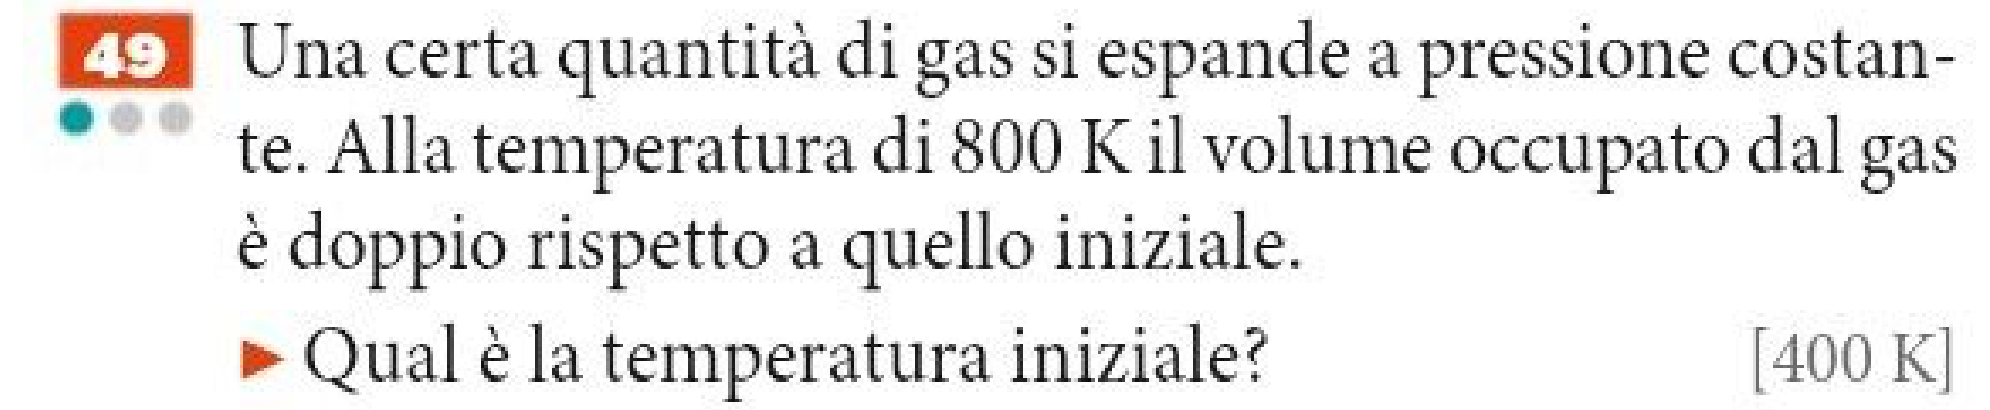
\includegraphics[width=0.85\linewidth]{immagini/es_49_espansione_isobara.png}

\vspace{0.3cm}
\raggedright
\textbf{Dati:}
\begin{itemize}
  \item Trasformazione isobara: $p = \text{costante}$;
  \item Volume iniziale del gas: $V_1$;
  \item Volume finale del gas: $V_2 = 2 \cdot V_1 \implies \dfrac{V_1}{V_2} = \dfrac{1}{2}$;
  \item Temperatura termodinamica finale: $T_2 = 800\,\text{K}$;
  \item Incognita: Temperatura termodinamica iniziale $T_1 = ?$.
\end{itemize}

\begin{figure}[H]
\centering
\begin{tikzpicture}[scale=0.88, >=stealth]
  \draw[->, thick, primaryBlue] (0, 0) -- (6.2, 0) node[below right, font=\small\sffamily] {$V \, [\text{m}^3]$};
  \draw[->, thick, primaryBlue] (0, 0) -- (0, 3.8) node[above left, font=\small\sffamily] {$p \, [\text{Pa}]$};
  \node[below left, primaryBlue] at (0, 0) {$O$};
  
  \coordinate (A) at (1.6, 2.4);
  \coordinate (B) at (4.4, 2.4);
  
  \draw[dashed, gray!80] (1.6, 0) node[below, font=\footnotesize] {$V_1$} -- (A) -- (0, 2.4) node[left, font=\footnotesize] {$p_1 = p_2 = p$};
  \draw[dashed, gray!80] (4.4, 0) node[below, font=\footnotesize] {$V_2 = 2V_1$} -- (B);
  
  \draw[very thick, accentRed] (A) -- (B);
  \draw[-{Latex[length=3mm]}, very thick, accentAmber] (2.7, 2.4) -- (3.3, 2.4) node[midway, above, font=\scriptsize\bfseries] {Espansione isobara};
  
  \fill[primaryBlue] (A) circle (2.5pt) node[above left, font=\footnotesize\bfseries] {$1(V_1, p)$};
  \fill[primaryBlue] (B) circle (2.5pt) node[above right, font=\footnotesize\bfseries] {$2(2V_1, p)$};
\end{tikzpicture}
\quad
\begin{tikzpicture}[scale=0.88, >=stealth]
  \draw[->, thick, primaryBlue] (0, 0) -- (6.2, 0) node[below right, font=\small\sffamily] {$T \, [\text{K}]$};
  \draw[->, thick, primaryBlue] (0, 0) -- (0, 3.8) node[above left, font=\small\sffamily] {$V \, [\text{m}^3]$};
  \node[below left, primaryBlue] at (0, 0) {$O$};
  
  \draw[thick, accentGreen!80!black, domain=0:5.2] plot (\x, {0.62*\x}) node[right, font=\footnotesize\bfseries] {$V = k \cdot T$};
  
  \coordinate (P1) at (2.0, {0.62*2.0});
  \coordinate (P2) at (4.0, {0.62*4.0});
  
  \draw[dashed, gray!80] (2.0, 0) node[below, font=\footnotesize] {$T_1 = 400\,\text{K}$} -- (P1) -- (0, {0.62*2.0}) node[left, font=\footnotesize] {$V_1$};
  \draw[dashed, gray!80] (4.0, 0) node[below, font=\footnotesize] {$T_2 = 800\,\text{K}$} -- (P2) -- (0, {0.62*4.0}) node[left, font=\footnotesize] {$V_2 = 2V_1$};
  
  \fill[primaryBlue] (P1) circle (2.5pt) node[above left, font=\footnotesize\bfseries] {Stato 1};
  \fill[primaryBlue] (P2) circle (2.5pt) node[above left, font=\footnotesize\bfseries] {Stato 2};
  \draw[-{Latex[length=3mm]}, very thick, accentAmber] (2.8, {0.62*2.8}) -- (3.3, {0.62*3.3});
\end{tikzpicture}
\caption{Rappresentazione cartesiana della trasformazione isobara dell'Esercizio 49: a sinistra nel piano di Clapeyron $(V, p)$ con il segmento orizzontale $1 \to 2$; a destra nel diagramma $(T, V)$ con la semiretta lineare passante per l'origine assoluta $O(0, 0)$.}
\label{fig:es49_grafici}
\end{figure}

\textbf{Risoluzione Formale:}\\
In base alla prima legge di Gay-Lussac espressa nella scala assoluta Kelvin, durante un'isobara il volume di un gas ideale \`e direttamente proporzionale alla temperatura termodinamica:
\[
\frac{V}{T} = \text{costante} \iff \frac{V_1}{T_1} = \frac{V_2}{T_2}
\]
Invertendo la relazione per determinare la temperatura iniziale $T_1$:
\[
T_1 = T_2 \cdot \frac{V_1}{V_2} = T_2 \cdot \frac{V_1}{2 \cdot V_1} = \frac{T_2}{2}
\]
Sostituendo il valore numerico fornito dal testo:
\[
T_1 = \frac{800\,\text{K}}{2} = \mathbf{400\,\text{K}}
\]
\textit{In gradi centigradi (Celsius):} $t_1 = T_1 - 273{,}15 = 400 - 273{,}15 = 126{,}85\,{^\circ}\text{C} \approx 127\,{^\circ}\text{C}$.

\begin{commento}[Interpretazione Cinetico-Molecolare del Fenomeno]
A pressione costante, l'espansione volumica al raddoppio ($V_2 = 2V_1$) riduce a met\`a la concentrazione volumica delle molecole ($N/V_2 = \frac{1}{2} N/V_1$). Affinch\'e la frequenza degli urti e l'impulso trasmesso alle pareti mantengano inalterata la pressione macroscopica $p = \frac{1}{3}\rho \langle v^2 \rangle$, l'energia cinetica media traslazionale $\langle E_c \rangle = \frac{3}{2}k_B T$ deve obbligatoriamente raddoppiare. Ci\`o impone che la temperatura termodinamica finale sia il doppio di quella iniziale ($T_2 = 2T_1 \implies T_1 = T_2 / 2$).
\end{commento}
\end{problema}

% ------------------------------------------------------------------------------
% ESERCIZIO 51
% ------------------------------------------------------------------------------
\begin{problema}[Esercizio 51 -- Cilindro con Pistone Libero e Dilatazione Isobara]
\centering
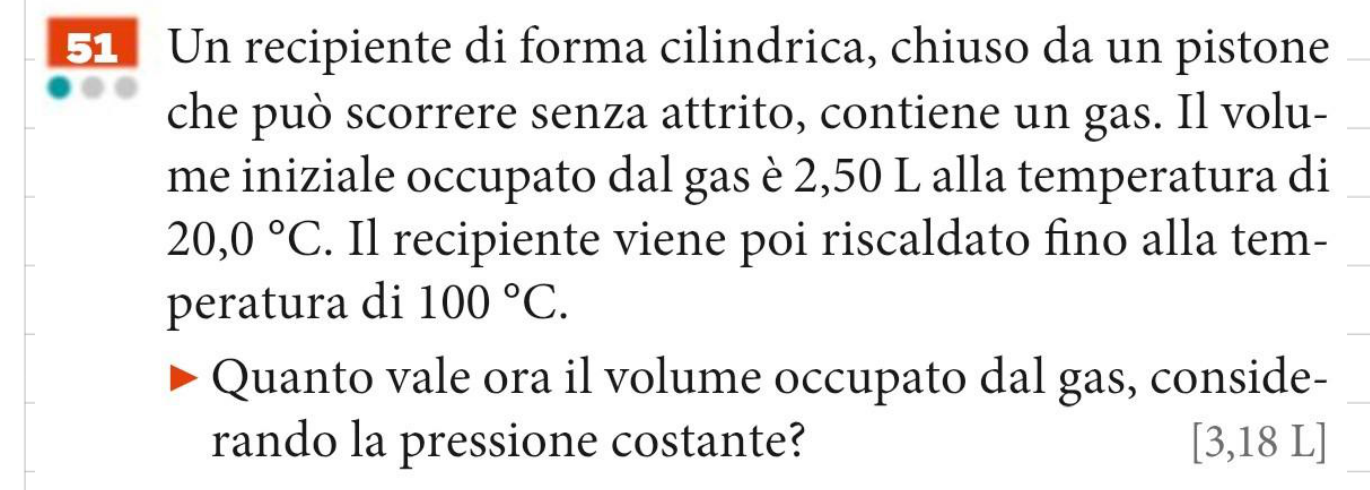
\includegraphics[width=0.75\linewidth]{immagini/es_51_pistone_cilindrico.png}

\vspace{0.3cm}
\raggedright
\textbf{Dati:}
\begin{itemize}
  \item Recipiente cilindrico con pistone a tenuta mobile e privo di attrito: $p = p_{\text{atm}} = \text{costante}$;
  \item Volume iniziale: $V_1 = 2{,}50\,\text{L} = 2{,}50 \cdot 10^{-3}\,\text{m}^3$;
  \item Temperatura centigrada iniziale: $t_1 = 20{,}0\,{^\circ}\text{C}$;
  \item Temperatura centigrada finale: $t_2 = 100{,}0\,{^\circ}\text{C}$;
  \item Incognita: Volume occupato alla temperatura finale $V_2 = ?$.
\end{itemize}

\begin{figure}[H]
\centering
\begin{tikzpicture}[scale=0.84, >=stealth]
  % Cilindro stato 1
  \draw[thick, primaryBlue] (0, 0) -- (0, 3.8) arc[start angle=180, end angle=0, x radius=1.2, y radius=0.3] -- (2.4, 0);
  \draw[thick, primaryBlue] (0, 0) arc[start angle=180, end angle=360, x radius=1.2, y radius=0.3];
  \draw[dashed, primaryBlue!60] (0, 0) arc[start angle=180, end angle=0, x radius=1.2, y radius=0.3];
  
  \fill[waterBlue!60, opacity=0.7] (0, 0) -- (0, 1.8) arc[start angle=180, end angle=360, x radius=1.2, y radius=0.3] -- (2.4, 0) arc[start angle=360, end angle=180, x radius=1.2, y radius=0.3];
  
  \fill[gray!40] (0, 1.8) arc[start angle=180, end angle=360, x radius=1.2, y radius=0.3] -- (2.4, 2.1) arc[start angle=0, end angle=180, x radius=1.2, y radius=0.3] -- cycle;
  \draw[thick, black!80] (0, 1.8) arc[start angle=180, end angle=360, x radius=1.2, y radius=0.3];
  \draw[thick, black!80] (0, 2.1) arc[start angle=180, end angle=360, x radius=1.2, y radius=0.3];
  \draw[thick, black!80] (0, 2.1) arc[start angle=180, end angle=0, x radius=1.2, y radius=0.3];
  \draw[thick, black!80] (0, 1.8) -- (0, 2.1);
  \draw[thick, black!80] (2.4, 1.8) -- (2.4, 2.1);
  
  \fill[gray!60] (1.1, 2.1) rectangle (1.3, 3.5);
  \draw[thick] (1.1, 2.1) rectangle (1.3, 3.5);
  
  \node[font=\footnotesize\bfseries, primaryBlue] at (1.2, 0.9) {$V_1 = 2{,}50\,\text{L}$};
  \node[font=\footnotesize\bfseries, primaryBlue] at (1.2, 0.4) {$T_1 = 293{,}15\,\text{K}$};
  \node[above, font=\small\sffamily\bfseries] at (1.2, 4.0) {Stato 1 ($20\,{^\circ}\text{C}$)};

  \draw[->, very thick, accentRed] (3.1, 1.8) -- (4.3, 1.8) node[midway, above, font=\scriptsize\bfseries] {Riscaldamento};
  \node[below, font=\scriptsize, accentRed] at (3.7, 1.7) {$\Delta Q > 0, \, p = \text{cost}$};

  \begin{scope}[xshift=5.0cm]
    \draw[thick, primaryBlue] (0, 0) -- (0, 3.8) arc[start angle=180, end angle=0, x radius=1.2, y radius=0.3] -- (2.4, 0);
    \draw[thick, primaryBlue] (0, 0) arc[start angle=180, end angle=360, x radius=1.2, y radius=0.3];
    \draw[dashed, primaryBlue!60] (0, 0) arc[start angle=180, end angle=0, x radius=1.2, y radius=0.3];
    
    \fill[waterBlue!60, opacity=0.7] (0, 0) -- (0, 2.6) arc[start angle=180, end angle=360, x radius=1.2, y radius=0.3] -- (2.4, 0) arc[start angle=360, end angle=180, x radius=1.2, y radius=0.3];
    
    \fill[gray!40] (0, 2.6) arc[start angle=180, end angle=360, x radius=1.2, y radius=0.3] -- (2.4, 2.9) arc[start angle=0, end angle=180, x radius=1.2, y radius=0.3] -- cycle;
    \draw[thick, black!80] (0, 2.6) arc[start angle=180, end angle=360, x radius=1.2, y radius=0.3];
    \draw[thick, black!80] (0, 2.9) arc[start angle=180, end angle=360, x radius=1.2, y radius=0.3];
    \draw[thick, black!80] (0, 2.9) arc[start angle=180, end angle=0, x radius=1.2, y radius=0.3];
    \draw[thick, black!80] (0, 2.6) -- (0, 2.9);
    \draw[thick, black!80] (2.4, 2.6) -- (2.4, 2.9);
    
    \fill[gray!60] (1.1, 2.9) rectangle (1.3, 3.8);
    \draw[thick] (1.1, 2.9) rectangle (1.3, 3.8);
    
    \node[font=\footnotesize\bfseries, primaryBlue] at (1.2, 1.4) {$V_2 = 3{,}18\,\text{L}$};
    \node[font=\footnotesize\bfseries, primaryBlue] at (1.2, 0.8) {$T_2 = 373{,}15\,\text{K}$};
    \node[above, font=\small\sffamily\bfseries] at (1.2, 4.0) {Stato 2 ($100\,{^\circ}\text{C}$)};
  \end{scope}
\end{tikzpicture}
\caption{Modello fisico del recipiente cilindrico con pistone mobile (Esercizio 51): l'assenza di attriti garantisce la pressione costante del gas ($p = p_{\text{atm}}$); l'innalzamento della temperatura causa la dilatazione volumica del gas con innalzamento del pistone da $V_1 = 2{,}50\,\text{L}$ a $V_2 = 3{,}18\,\text{L}$.}
\label{fig:cilindro_pistone_es51}
\end{figure}

\textbf{Metodo 1: Risoluzione mediante Temperatura Assoluta Kelvin (Consigliato)}\\
Convertiamo le temperature centigrade nella scala termodinamica assoluta:
\[
T_1 = t_1 + 273{,}15 = 20{,}0 + 273{,}15 = 293{,}15\,\text{K}
\]
\[
T_2 = t_2 + 273{,}15 = 100{,}0 + 273{,}15 = 373{,}15\,\text{K}
\]
Per la prima legge di Gay-Lussac:
\[
\frac{V_1}{T_1} = \frac{V_2}{T_2} \implies V_2 = V_1 \cdot \frac{T_2}{T_1}
\]
Sostituendo i valori numerici:
\[
V_2 = 2{,}50\,\text{L} \cdot \frac{373{,}15\,\text{K}}{293{,}15\,\text{K}} = 2{,}50\,\text{L} \cdot 1{,}272898 \approx \mathbf{3{,}182\,\text{L}} \approx \mathbf{3{,}18\,\text{L}}
\]

\textbf{Metodo 2: Risoluzione con la Legge Centigrada Storica (con Determinazione di $V_0$)}\\
La formulazione centigrada riferita alla temperatura convenzionale di $0\,{^\circ}\text{C}$ stabilisce:
\[
V(t) = V_0 (1 + \alpha \cdot t), \qquad \text{con } \alpha = \frac{1}{273{,}15\,{^\circ}\text{C}} \approx 0{,}003661\,{^\circ}\text{C}^{-1}
\]
Dallo stato iniziale $V_1 = V(t_1)$ ricaviamo il volume teorico a $0\,{^\circ}\text{C}$ ($V_0$):
\[
V_0 = \frac{V_1}{1 + \alpha t_1} = \frac{2{,}50\,\text{L}}{1 + \dfrac{20{,}0}{273{,}15}} = \frac{2{,}50\,\text{L}}{1{,}07322} \approx 2{,}3294\,\text{L}
\]
Calcoliamo ora il volume $V_2$ alla temperatura $t_2 = 100{,}0\,{^\circ}\text{C}$:
\[
V_2 = V_0 (1 + \alpha t_2) = 2{,}3294\,\text{L} \cdot \left(1 + \frac{100{,}0}{273{,}15}\right) = 2{,}3294\,\text{L} \cdot 1{,}3661 \approx \mathbf{3{,}182\,\text{L}} \approx \mathbf{3{,}18\,\text{L}}
\]
La perfetta concordanza tra i due metodi conferma la coerenza della termometria dei gas ideali.
\end{problema}

% ------------------------------------------------------------------------------
% ESERCIZIO 52
% ------------------------------------------------------------------------------
\begin{problema}[Esercizio 52 -- Determinazione Sperimentale del Coefficiente di Dilatazione $\alpha$]
\centering
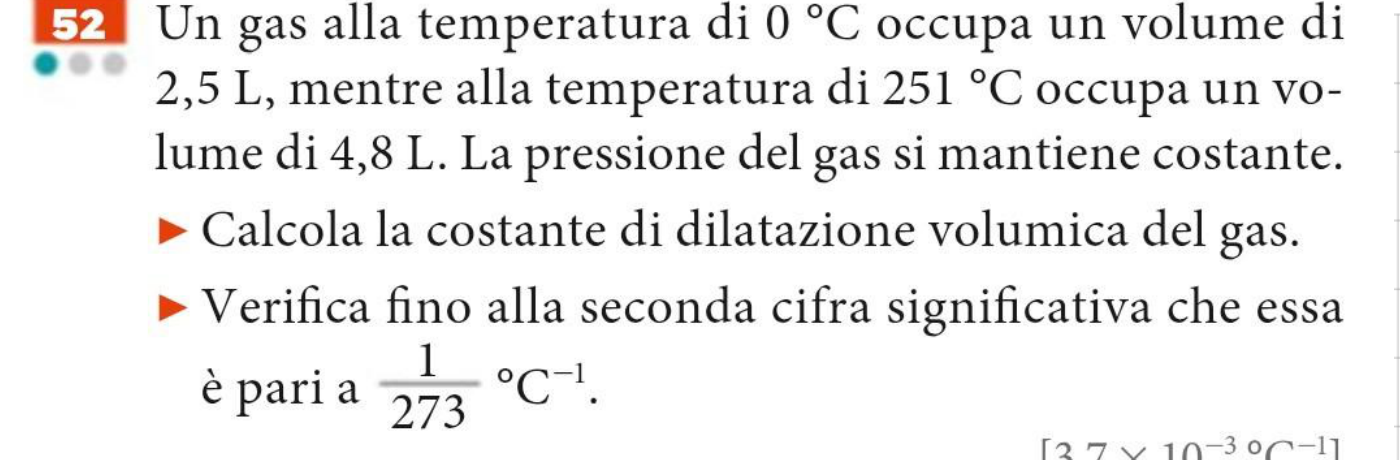
\includegraphics[width=0.75\linewidth]{immagini/es_52_dilatazione_volumica.png}

\vspace{0.3cm}
\raggedright
\textbf{Dati:}
\begin{itemize}
  \item Pressione costante del gas: $p = \text{costante}$;
  \item Volume alla temperatura di riferimento di $0\,{^\circ}\text{C}$: $t_0 = 0\,{^\circ}\text{C} \implies V_0 = 2{,}5\,\text{L}$;
  \item Volume alla temperatura riscaldata: $t_1 = 251\,{^\circ}\text{C} \implies V_1 = 4{,}8\,\text{L}$;
  \item Richieste del testo:
    \begin{enumerate}
      \item Calcolare la costante di dilatazione volumica $\alpha$ del gas;
      \item Verificare fino alla seconda cifra significativa che essa \`e pari a $\dfrac{1}{273}\,{^\circ}\text{C}^{-1}$.
    \end{enumerate}
\end{itemize}

\textbf{1. Isolamento Algebrico del Coefficiente $\alpha$:}\\
Partiamo dalla legge di Gay-Lussac riferita a $0\,{^\circ}\text{C}$:
\[
V_1 = V_0 (1 + \alpha \cdot t_1)
\]
Applichiamo i principi di equivalenza delle equazioni algebriche:
\begin{enumerate}[label=\alph*)]
  \item Propriet\`a simmetrica dell'uguaglianza:
  \[
  V_0 (1 + \alpha \cdot t_1) = V_1
  \]
  \item Secondo principio di equivalenza (divisione per $V_0 \neq 0$):
  \[
  1 + \alpha \cdot t_1 = \frac{V_1}{V_0}
  \]
  \item Primo principio di equivalenza (trasposizione dell'unit\`a):
  \[
  \alpha \cdot t_1 = \frac{V_1}{V_0} - 1 = \frac{V_1 - V_0}{V_0}
  \]
  \item Isolamento dell'incognita $\alpha$ (divisione per $t_1 \neq 0$):
  \[
  \alpha = \frac{1}{t_1} \cdot \left(\frac{V_1}{V_0} - 1\right) = \frac{V_1 - V_0}{V_0 \cdot t_1}
  \]
\end{enumerate}

\textbf{2. Sostituzione Numerica e Calcolo del Reciproco:}\\
Inserendo i dati sperimentali forniti:
\[
\alpha = \frac{1}{251\,{^\circ}\text{C}} \cdot \left(\frac{4{,}8\,\text{L}}{2{,}5\,\text{L}} - 1\right) = \frac{1}{251\,{^\circ}\text{C}} \cdot (1{,}92 - 1) = \frac{0{,}92}{251\,{^\circ}\text{C}} \approx \mathbf{0{,}0036653\,{^\circ}\text{C}^{-1}}
\]
Esprimiamo il risultato sotto forma di frazione con numeratore unitario $\alpha = \dfrac{1}{1/\alpha}$:
\[
\frac{1}{\alpha} = \frac{251\,{^\circ}\text{C}}{0{,}92} \approx 272{,}826\,{^\circ}\text{C} \implies \alpha = \frac{1}{272{,}8\,{^\circ}\text{C}}
\]

\textbf{3. Verifica Rigorosa delle Cifre Significative (2 c.s.):}\\
I dati del volume misurati in laboratorio ($V_0 = 2{,}5\,\text{L}$ e $V_1 = 4{,}8\,\text{L}$) possiedono due cifre significative.
Arrotondando il denominatore a due cifre significative:
\[
272{,}8\,{^\circ}\text{C} \approx \mathbf{2{,}7 \cdot 10^2\,{^\circ}\text{C}} \approx 270\,{^\circ}\text{C}
\]
Ed esprimendo il valore numerico di $\alpha$ in notazione scientifica a 2 cifre significative:
\[
\alpha = 0{,}0036653\,{^\circ}\text{C}^{-1} \approx \mathbf{3{,}7 \cdot 10^{-3}\,{^\circ}\text{C}^{-1}}
\]
Confrontando questo responso con il reciproco teorico di $273$:
\[
\frac{1}{273} \approx 0{,}0036630\,\dots \approx \mathbf{3{,}7 \cdot 10^{-3}\,{^\circ}\text{C}^{-1}}
\]
La verifica sperimentale fino alla seconda cifra significativa risulta pienamente soddisfatta e concordante con le previsioni del modello cinetico dei gas ideali.
\end{problema}

% ------------------------------------------------------------------------------
% ESERCIZIO 65
% ------------------------------------------------------------------------------
\begin{problema}[Esercizio 65 -- Espansione Isobara Percentuale]
\centering
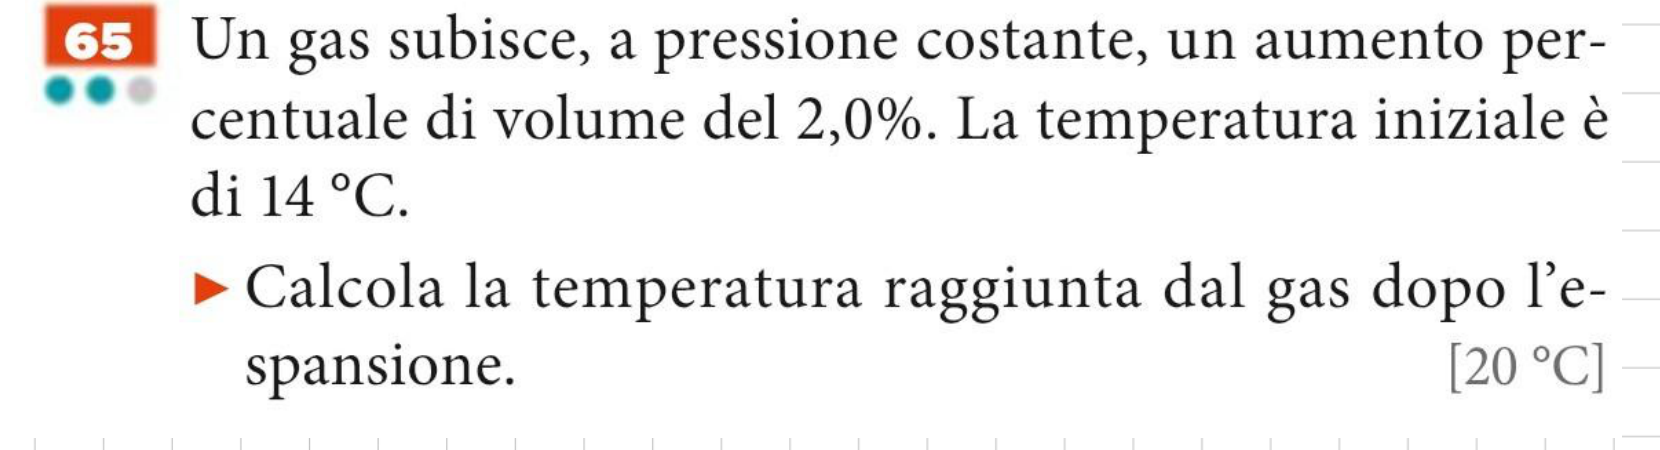
\includegraphics[width=0.75\linewidth]{immagini/es_65_espansione_isobara.png}

\vspace{0.3cm}
\raggedright
\textbf{Dati:}
\begin{itemize}
  \item Trasformazione isobara: $p = \text{costante}$;
  \item Aumento percentuale di volume: $\Delta V / V_1 = 2{,}0\% = 0{,}020$;
  \item Temperatura iniziale: $t_1 = 14\,{^\circ}\text{C}$.
\end{itemize}

\textbf{Metodo 1: Risoluzione mediante Temperatura Assoluta Kelvin}\\
Convertiamo la temperatura iniziale nella scala assoluta:
\[
T_1 = t_1 + 273{,}15 = 14 + 273{,}15 = 287{,}15\,\text{K}
\]
Il volume finale \`e legato al volume iniziale da:
\[
V_2 = V_1 + 0{,}020 \cdot V_1 = 1{,}020 \cdot V_1 = \frac{51}{50} V_1
\]
Per la prima legge di Gay-Lussac a pressione costante:
\[
\frac{V_1}{T_1} = \frac{V_2}{T_2} \implies T_2 = T_1 \cdot \frac{V_2}{V_1} = 287{,}15\,\text{K} \cdot 1{,}020 \approx 292{,}89\,\text{K}
\]
Riconvertendo in gradi Celsius:
\[
t_2 = T_2 - 273{,}15 = 292{,}89 - 273{,}15 \approx \mathbf{19{,}74\,{^\circ}\text{C}} \approx \mathbf{20\,{^\circ}\text{C}}
\]

\textbf{Metodo 2: Risoluzione con la Formula Centigrada Classica}\\
Scriviamo la dilatazione per lo stato iniziale e finale rispetto allo zero centigrado:
\[
V_1 = V_0 (1 + \alpha t_1), \qquad V_2 = V_0 (1 + \alpha t_2)
\]
Eseguendo il rapporto membro a membro per eliminare $V_0$:
\[
\frac{V_1}{V_2} = \frac{1 + \alpha t_1}{1 + \alpha t_2} \implies \frac{50}{51} = \frac{1 + \alpha t_1}{1 + \alpha t_2}
\]
Invertendo ed esplicitando $\alpha t_2$:
\[
1 + \alpha t_2 = \frac{51}{50}(1 + \alpha t_1) \implies \alpha t_2 = \frac{51}{50}(1 + \alpha t_1) - 1 = \frac{1 + 51 \alpha t_1}{50}
\]
Moltiplicando per $1/\alpha = 273{,}15\,{^\circ}\text{C}$:
\[
t_2 = \frac{1}{\alpha} \left(\frac{1 + 51 \alpha t_1}{50}\right) = 273{,}15 \cdot \left(\frac{1 + 51 \cdot 0{,}00366 \cdot 14}{50}\right) = 273{,}15 \cdot \frac{3{,}613}{50} \approx \mathbf{19{,}74\,{^\circ}\text{C}} \approx \mathbf{20\,{^\circ}\text{C}}
\]
I due metodi conducono al medesimo risultato sperimentale, confermando la coerenza del modello di dilatazione dei gas.
\end{problema}

% ------------------------------------------------------------------------------
% ESERCIZIO 66
% ------------------------------------------------------------------------------
\begin{problema}[Esercizio 66 -- Variazione Percentuale di Pressione in Trasformazione Isocora]
\centering
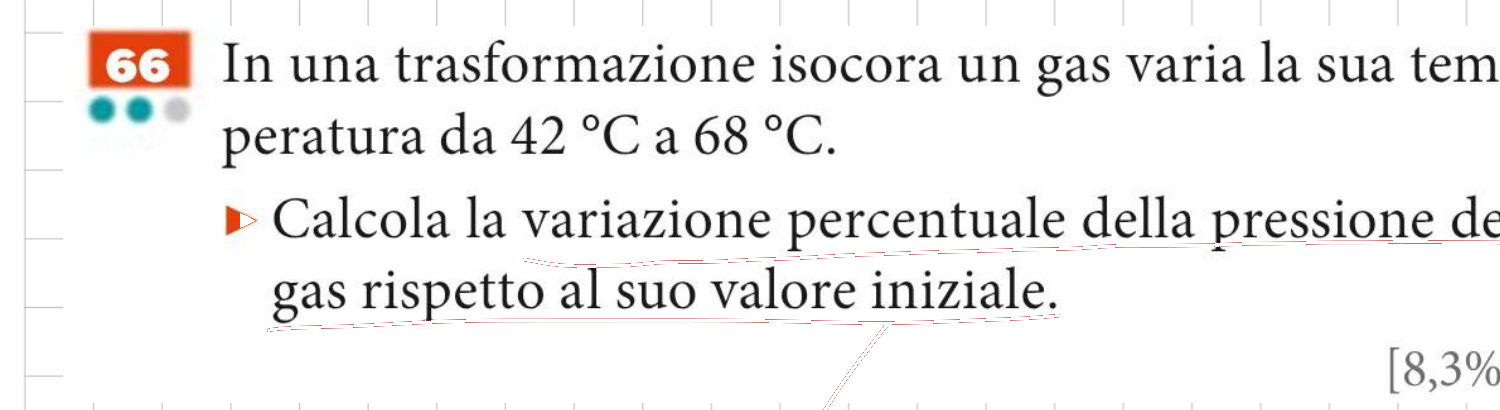
\includegraphics[width=0.75\linewidth]{immagini/es_66_variazione_pressione_isocora.png}

\vspace{0.3cm}
\raggedright
\textbf{Dati:}
\begin{itemize}
  \item Trasformazione isocora: volume costante ($V = \text{costante}$);
  \item Temperatura iniziale: $t_1 = 42\,{^\circ}\text{C}$;
  \item Temperatura finale: $t_2 = 68\,{^\circ}\text{C}$;
  \item Incognita richiesta dal libro: Variazione percentuale della pressione del gas rispetto al suo valore iniziale:
  \[
  \frac{\Delta p}{p_1} \cdot 100\% = \left(\frac{p_2 - p_1}{p_1}\right) \cdot 100\% = \left(\frac{p_2}{p_1} - 1\right) \cdot 100\%
  \]
\end{itemize}

\textbf{Metodo 1: Risoluzione mediante Temperatura Assoluta Kelvin (Metodo Diretto ed Esatto)}\\
Convertiamo immediatamente le temperature centigrade nella scala termodinamica Kelvin:
\[
T_1 = t_1 + 273{,}15 = 42 + 273{,}15 = 315{,}15\,\text{K}
\]
\[
T_2 = t_2 + 273{,}15 = 68 + 273{,}15 = 341{,}15\,\text{K}
\]
In una trasformazione isocora, la seconda legge di Gay-Lussac stabilisce la proporzionalit\`a diretta tra pressione e temperatura assoluta:
\[
\frac{p_1}{T_1} = \frac{p_2}{T_2} \iff \frac{p_2}{p_1} = \frac{T_2}{T_1}
\]
La variazione relativa percentuale si esprime dunque direttamente attraverso il rapporto delle temperature Kelvin:
\[
\frac{\Delta p}{p_1} \cdot 100\% = \left(\frac{T_2}{T_1} - 1\right) \cdot 100\% = \frac{T_2 - T_1}{T_1} \cdot 100\%
\]
Sostituendo i valori numerici:
\[
\frac{\Delta p}{p_1} \cdot 100\% = \frac{341{,}15\,\text{K} - 315{,}15\,\text{K}}{315{,}15\,\text{K}} \cdot 100\% = \frac{26\,\text{K}}{315{,}15\,\text{K}} \cdot 100\% \approx 0{,}082500 \cdot 100\% = \mathbf{8{,}25\%} \approx \mathbf{8{,}3\%}
\]
Il valore ottenuto coincide perfettamente con il risultato ufficiale del libro di testo ($[8{,}3\%]$).

\textbf{Metodo 2: Risoluzione con il Sistema Centigrado di Gay-Lussac}\\
Impostiamo il sistema delle pressioni riferite alla pressione $p_0$ a $0\,{^\circ}\text{C}$:
\[
\begin{cases}
p_1 = p_0 (1 + \alpha \cdot t_1) \\
p_2 = p_0 (1 + \alpha \cdot t_2)
\end{cases}
\]
Eseguiamo la divisione membro a membro, semplificando il fattore comune $p_0$:
\[
\frac{p_2}{p_1} = \frac{p_0 (1 + \alpha t_2)}{p_0 (1 + \alpha t_1)} = \frac{1 + \alpha t_2}{1 + \alpha t_1}
\]
Sottraendo $1$ ad entrambi i membri per ottenere la variazione relativa:
\[
\frac{p_2}{p_1} - 1 = \frac{1 + \alpha t_2}{1 + \alpha t_1} - 1 = \frac{1 + \alpha t_2 - (1 + \alpha t_1)}{1 + \alpha t_1} = \frac{\alpha (t_2 - t_1)}{1 + \alpha t_1}
\]
Poich\'e $\alpha = \frac{1}{T_0}$ con $T_0 = 273{,}15\,\text{K}$, moltiplicando numeratore e denominatore per $T_0$:
\[
\frac{\Delta p}{p_1} = \frac{\Delta t}{T_0 + t_1} = \frac{68 - 42}{273{,}15 + 42} = \frac{26}{315{,}15} \approx \mathbf{8{,}3\%}
\]

\begin{avviso}[Tranello del Calcolo Numerico: Gli Arrotondamenti Intermedi Precoci]
Nel calcolo numerico centigrado, approssimando precocemente i singoli binomi a poche cifre decimali prima della divisione:
\[
1 + \alpha t_2 = 1 + \frac{68}{273{,}15} \approx 1{,}2489 \longrightarrow \text{troncato a } 1{,}24
\]
\[
1 + \alpha t_1 = 1 + \frac{42}{273{,}15} \approx 1{,}1537 \longrightarrow \text{troncato a } 1{,}15
\]
si otterrebbe:
\[
\left(\frac{1{,}24}{1{,}15} - 1\right) \cdot 100\% = (1{,}0782 - 1) \cdot 100\% \approx \mathbf{7{,}8\%}
\]
Questo scostamento (da $8{,}3\%$ a $7{,}8\%$) \`e dovuto alla \textbf{cancellazione numerica}: quando si sottrae l'unit\`a $(p_2/p_1 - 1)$, la parte intera si elide e l'errore introdotto sui decimali si amplifica enormemente sulla percentuale finale. \'E fondamentale mantenere la forma frazionaria esatta fino al calcolo finale o impiegare direttamente le temperature assolute Kelvin.
\end{avviso}
\end{problema}

% ==============================================================================
% CAPITOLO 8: L'EQUAZIONE DI STATO DEL GAS PERFETTO
% ==============================================================================
\chapter{L'Equazione di Stato del Gas Perfetto e la Costante Universale \texorpdfstring{$R$}{R}}

\section{Il Modello Microscopico e Macroscopico del Gas Perfetto}
Nelle lezioni precedenti abbiamo analizzato il comportamento dei gas attraverso trasformazioni termodinamiche particolari, mantenendo costante una delle tre variabili di stato macroscopiche: la temperatura (legge di Boyle), la pressione (prima legge di Gay-Lussac) o il volume (seconda legge di Gay-Lussac).

Tuttavia, nella realt\`a fisica e nelle applicazioni ingegneristiche e chimiche, le tre grandezze di stato ($p$, $V$, $T$) variano frequentemente in modo simultaneo. Per descrivere lo stato di equilibrio di un gas in qualunque condizione, la fisica introduce il modello teorico del \textbf{gas perfetto} (o gas ideale).

\begin{definizione}[Gas Perfetto o Gas Ideale]
Un gas reale segue con eccellente approssimazione il modello ideale di \textbf{gas perfetto} quando soddisfa le seguenti tre condizioni sperimentali e microscopiche:
\begin{enumerate}[label=\textbf{\arabic*.}]
    \item \textbf{Bassa densit\`a e rarefazione:} Il gas si trova a una pressione sufficientemente bassa, tale che la distanza media tra le molecole sia molto grande rispetto alle dimensioni delle molecole stesse.
    \item \textbf{Temperatura lontana dalla liquefazione:} La temperatura assoluta $T$ del gas \`e nettamente superiore alla sua temperatura critica e alla temperatura di transizione alla fase liquida ($T \gg T_{\text{liq}}$), scongiurando la condensazione.
    \item \textbf{Volume proprio trascurabile e urti elastici:} Le molecole e gli atomi possono essere trattati come masse puntiformi il cui volume proprio \`e del tutto trascurabile rispetto al volume totale $V$ del recipiente ($V_{\text{molecole}} \ll V_{\text{recipiente}}$). Le interazioni reciproche a distanza sono nulle (assenza di forze di Van der Waals o dipolari): le particelle interagiscono unicamente tramite urti perfettamente elastici tra di loro e contro le pareti del contenitore.
\end{enumerate}
\end{definizione}

Nelle ordinarie condizioni ambiente (pressione atmosferica di $1\,\text{atm}$ e temperature prossime a $20\,{^\circ}\text{C}$), i gas atmosferici comuni (quali l'azoto $\text{N}_2$, l'ossigeno $\text{O}_2$, l'elio $\text{He}$ e l'idrogeno $\text{H}_2$) manifestano scostamenti inferiori allo $0{,}1\%$ rispetto al comportamento ideale.

\section{Il Principio di Avogadro e la Quantit\`a di Sostanza}
Il fondamento teorico che consente di unificare le variabili meccaniche ($p, V$) con quella termica ($T$) e con la quantit\`a di materia \`e il celebre principio formulato dal chimico e fisico piemontese Amedeo Avogadro nel 1811:

\begin{leggefisica}[Legge o Principio di Avogadro]
Volumi uguali di gas diversi, mantenuti nelle medesime condizioni di temperatura assoluta $T$ e di pressione $p$, contengono esattamente lo stesso numero di molecole $N$ e, di conseguenza, lo stesso numero di moli $n$.
\[
V \propto n \quad (\text{a } p = \text{costante e } T = \text{costante})
\]
\end{leggefisica}

Questo principio fondamentale sancisce che le propriet\`a termodinamiche macroscopiche di un gas perfetto non dipendono dalla natura chimica specifica del gas (se si tratti di ossigeno biatomico, elio monoatomico o anidride carbonica), bens\`i unicamente dal numero totale di particelle presenti nel sistema.

\section{L'Equazione di Stato dei Gas Perfetti (Legge di Clapeyron)}
Combinando il principio di Avogadro con le tre leggi sperimentali (Boyle e Gay-Lussac), si ottiene l'equazione fondamentale che correla in modo univoco tutte le coordinate termodinamiche di stato:

\begin{leggefisica}[Equazione di Stato del Gas Perfetto]
Lo stato di equilibrio termodinamico di $n$ moli di un gas ideale \`e regolato dall'equazione:
\begin{equation}
\bm{p \cdot V = n \cdot R \cdot T}
\end{equation}
in cui:
\begin{itemize}[label=$\diamond$]
    \item $p$ \`e la pressione assoluta esercitata dal gas, espressa in \textbf{Pascal} ($\text{Pa} = \text{N}/\text{m}^2$);
    \item $V$ \`e il volume occupato dal gas, espresso in \textbf{metri cubi} ($\text{m}^3$);
    \item $n$ \`e la quantit\`a di sostanza, espressa in \textbf{moli} ($\text{mol}$);
    \item $T$ \`e la temperatura assoluta, rigorosamente espressa in \textbf{Kelvin} ($\text{K}$);
    \item $R$ \`e la \textbf{costante universale dei gas perfetti}.
\end{itemize}
\end{leggefisica}

\subsection*{Analisi Dimensionale del Prodotto $p \cdot V$}
\`E di fondamentale rilevanza fisica esaminare la natura dimensionale del membro sinistro dell'equazione di stato:
\[
[p \cdot V] = [\text{Pa}] \cdot [\text{m}^3] = \left[\frac{\text{N}}{\text{m}^2}\right] \cdot [\text{m}^3] = [\text{N} \cdot \text{m}] = [\text{Joule}]
\]
Il prodotto $p \cdot V$ possiede le dimensioni fisiche di un'\textbf{energia} o di un \textbf{lavoro meccanico} ($\text{J}$). Quando un gas a pressione $p$ compie un'espansione isobarica variando il proprio volume di $\Delta V$, il lavoro compiuto contro l'ambiente esterno \`e proprio dato da $W = p \cdot \Delta V$. Dunque, $nRT$ quantifica l'energia termica associata al moto traslazionale delle molecole nel recipiente.

\section{La Costante Universale \texorpdfstring{$R$}{R} e il Confronto tra Unit\`a del SI e Unit\`a Chimiche}
Dall'equazione di stato si ricava l'espressione esplicita per la costante universale $R$:
\begin{equation}
R = \frac{p \cdot V}{n \cdot T}
\end{equation}
Nel Sistema Internazionale di unit\`a di misura:
\[
[R] = \frac{\text{Pa} \cdot \text{m}^3}{\text{mol} \cdot \text{K}} = \frac{\text{J}}{\text{mol} \cdot \text{K}}
\]
Il valore numerico misurato sperimentalmente con elevatissima precisione \`e:
\begin{equation}
\bm{R = 8{,}31446\,\frac{\text{J}}{\text{mol} \cdot \text{K}} \approx 8{,}31\,\frac{\text{J}}{\text{mol} \cdot \text{K}}}
\end{equation}

\subsection*{Espressione di $R$ nelle Unit\`a Pratiche della Chimica: $\text{L} \cdot \text{atm} / (\text{mol} \cdot \text{K})$}
Nella pratica dei laboratori chimici e negli esercizi applicativi, la pressione \`e frequentemente misurata in atmosfere ($\text{atm}$) e il volume in litri ($\text{L} = \text{dm}^3$). 
Dimostriamo come si effettua la rigorosa conversione:
\begin{align*}
1\,\text{atm} &= 101\,325\,\text{Pa} \\
1\,\text{L} &= 1\,\text{dm}^3 = 10^{-3}\,\text{m}^3
\end{align*}
Pertanto, il fattore di conversione energetico tra litri-atmosfere e Joule vale:
\[
1\,\text{L} \cdot \text{atm} = \left(10^{-3}\,\text{m}^3\right) \times \left(101\,325\,\frac{\text{N}}{\text{m}^2}\right) = 101{,}325\,\text{N} \cdot \text{m} = \mathbf{101{,}325\,\text{J}}
\]
Esprimendo la costante universale $R$ in queste unit\`a pratiche:
\[
R = \frac{8{,}31446\,\frac{\text{J}}{\text{mol} \cdot \text{K}}}{101{,}325\,\frac{\text{J}}{\text{L} \cdot \text{atm}}} \approx \mathbf{0{,}082057\,\frac{\text{L} \cdot \text{atm}}{\text{mol} \cdot \text{K}} \approx 0{,}0821\,\frac{\text{L} \cdot \text{atm}}{\text{mol} \cdot \text{K}}}
\]

\begin{avviso}[Scelta della Costante $R$ e Coerenza delle Unit\`a di Misura]
Uno degli errori pi\`u frequenti commessi nella risoluzione dei problemi di termodinamica riguarda l'incoerenza tra le unit\`a di misura delle variabili e il valore di $R$ adottato:
\begin{itemize}
    \item Se si utilizza $\bm{R = 8{,}31\,\text{J}/(\text{mol} \cdot \text{K})}$, la pressione deve essere tassativamente in \textbf{Pascal} ($\text{Pa}$) e il volume in \textbf{metri cubi} ($\text{m}^3$).
    \item Se si impiega $\bm{R = 0{,}0821\,(\text{L} \cdot \text{atm})/(\text{mol} \cdot \text{K})}$, la pressione deve essere in \textbf{atmosfere} ($\text{atm}$) e il volume in \textbf{litri} ($\text{L}$).
    \item In \textbf{entrambi i casi}, la temperatura $T$ DEVE essere rigorosamente convertita nella scala assoluta \textbf{Kelvin} ($T = t + 273{,}15$). L'inserimento diretto di gradi Celsius nell'equazione di stato invalida irrimediabilmente il calcolo!
\end{itemize}
\end{avviso}

\subsection*{Applicazione Notevole: Il Volume Molare Standard (STP)}
Determiniamo il volume occupato da una mole ($n = 1\,\text{mol}$) di un qualsiasi gas ideale nelle condizioni standard di temperatura e pressione (\textbf{STP}, \textit{Standard Temperature and Pressure}: $T = 0\,{^\circ}\text{C} = 273{,}15\,\text{K}$ e $p = 1{,}00\,\text{atm}$):
\[
V_0 = \frac{n \cdot R \cdot T}{p} = \frac{1\,\text{mol} \cdot 0{,}0821\,\frac{\text{L}\cdot\text{atm}}{\text{mol}\cdot\text{K}} \cdot 273{,}15\,\text{K}}{1{,}00\,\text{atm}} \approx \mathbf{22{,}414\,\text{L} \approx 22{,}4\,\text{L}}
\]
Questo risultato fondamentale conferma che \textit{una mole di qualunque gas perfetto occupa un volume di circa $22{,}4\,\text{litri}$ a $0\,{^\circ}\text{C}$ e $1\,\text{atm}$}.

\section{Deduzione delle Tre Leggi Storiche dall'Equazione di Stato}
L'equazione di stato unifica e sintetizza in una sola legge generale l'intero corpus delle leggi empiriche scoperte nel XVII, XVIII e XIX secolo:

\begin{enumerate}[label=\textbf{\arabic*.}]
    \item \textbf{Legge di Boyle (Isoterma, $T = \text{costante}$, $n = \text{costante}$):}
    \[
    p \cdot V = \underbrace{n \cdot R \cdot T}_{\text{costante}} \implies \bm{p \cdot V = \text{costante}} \iff p_1 V_1 = p_2 V_2
    \]
    La pressione e il volume sono grandezze inversamente proporzionali. Nel piano di Clapeyron $(V, p)$, la curva rappresentativa \`e un ramo di iperbole equilatera.

    \item \textbf{Prima Legge di Gay-Lussac o Legge di Charles (Isobara, $p = \text{costante}$, $n = \text{costante}$):}
    \[
    \frac{V}{T} = \underbrace{\frac{n \cdot R}{p}}_{\text{costante}} \implies \bm{\frac{V}{T} = \text{costante}} \iff \frac{V_1}{T_1} = \frac{V_2}{T_2}
    \]
    Il volume e la temperatura assoluta sono direttamente proporzionali. Esprimendo $T$ rispetto a $0\,{^\circ}\text{C}$ ($T = T_0 + t$ con $\alpha = 1/T_0$):
    \[
    V(t) = \frac{nR}{p}(T_0 + t) = \frac{nRT_0}{p}\left(1 + \frac{t}{T_0}\right) = V_0(1 + \alpha t)
    \]
    ritrovando esattamente la formulazione empirica centigrada.

    \item \textbf{Seconda Legge di Gay-Lussac (Isocora, $V = \text{costante}$, $n = \text{costante}$):}
    \[
    \frac{p}{T} = \underbrace{\frac{n \cdot R}{V}}_{\text{costante}} \implies \bm{\frac{p}{T} = \text{costante}} \iff \frac{p_1}{T_1} = \frac{p_2}{T_2}
    \]
    La pressione e la temperatura assoluta sono direttamente proporzionali. Nel piano di Clapeyron centigrado si ritrova:
    \[
    p(t) = p_0(1 + \alpha t)
    \]
\end{enumerate}

\begin{table}[H]
\centering
\small
\renewcommand{\arraystretch}{1.4}
\begin{tabularx}{\textwidth}{l p{4.2cm} X l}
\toprule
\textbf{Trasformazione} & \textbf{Grandezze Costanti} & \textbf{Relazione Termodinamica} & \textbf{Legge Storica} \\
\midrule
\textbf{Isoterma} & Temperatura ($T = \text{cost}$), moli $n$ & $p \cdot V = \text{costante} \implies p_1 V_1 = p_2 V_2$ & Boyle (1662) \\
\textbf{Isobara} & Pressione ($p = \text{cost}$), moli $n$ & $\dfrac{V}{T} = \text{costante} \implies \dfrac{V_1}{T_1} = \dfrac{V_2}{T_2}$ & 1\textsuperscript{a} Gay-Lussac (1802) \\
\textbf{Isocora} & Volume ($V = \text{cost}$), moli $n$ & $\dfrac{p}{T} = \text{costante} \implies \dfrac{p_1}{T_1} = \dfrac{p_2}{T_2}$ & 2\textsuperscript{a} Gay-Lussac (1802) \\
\textbf{Generale} & Moli $n = \text{cost}$ ($p, V, T$ variabili) & $\dfrac{p \cdot V}{T} = n \cdot R = \text{costante}$ & Clapeyron (1834) \\
\bottomrule
\end{tabularx}
\caption{Quadro sinottico comparativo delle trasformazioni ideali ricavate dall'equazione di stato.}
\end{table}

\end{document}
